% EN48 c03 | 原书 p.23–43（PDF 32–52） | 第 1 章 §1.4–1.5
% 骨架文件：标题行已设定，正文由译者填写。每页起首用 % ===== 原书 p.N ===== 注释标记。
% 边界说明：p.23 上部的 Corollary 1.3.29 与 Remark 1.3.30 归 c02；本块从 §1.4 起。
\subsection{A 侧流形}

% ===== 原书 p.23 =====
我们已经有环簇背景，下一步是描述构造 $\tilde Y$ 的多面体所用的工具。对合适的全纯函数
$v_0$，$(Y,v_0)$ 应当与 $H=\Sigma_2\subset V$ 互为镜像；因此可以预期，该多面体由亏格 $2$
曲线的信息构造。对定义截面 $s$ 取热带化，就能从中提取组合数据。

\medskip\noindent\textbf{theta 函数的热带化}\par

\begin{definition}[热带化（Tropicalization）]\label{def:tropicalization}
设 $f(x)=\sum_{a\in A\subset\Z^n}c_ax^a\tau^{\rho(a)}$。令 $\xi=(\xi_1,\dots,\xi_n)$
是由
\[
|x_i|=\tau^{-\xi_i}
\]
定义的对数坐标（Log coordinates）。则
\[
f=\sum_a c_a\Bigl(\frac{x}{|x|}\Bigr)^a\tau^{\rho(a)-\ip{a}{\xi}}.
\]
特别地，热带极限对应 $\tau\to0$，也就是重新缩放 $|x_i|$，使 $\xi_i$ 保持不变。当
$\tau\to0$ 时，$f$ 的首项是 $\tau$ 的指数最小的那一项。$f$ 的热带化取该指数的相反数，
即
\[
\operatorname{Trop}(f):=-\min_{a\in A}\bigl(\rho(a)-\ip{a}{\xi}\bigr)
=\max_{a\in A}\bigl(\ip{a}{\xi}-\rho(a)\bigr).
\]
\end{definition}

\transnote{「取负号」是为了让 $|x_i|=\tau^{-\xi_i}$ 真正成为对数坐标：$\tau\to0$ 时
$\tau$ 的指数最小的项占优，取相反数后，它成为 $\xi$ 的仿射函数。于是
$\operatorname{Trop}(f)$ 是仿射函数的上包络，自动是凸的分段线性函数。}

% ===== 原书 p.24 =====
\begin{claim}\label{clm:periodicity}
设 $s$ 为上述 theta 函数。其热带化 $\varphi:=\operatorname{Trop}s$ 满足如下周期性质
\begin{equation}\label{eq:1-10}
\varphi(\xi+\tilde\gamma)=\varphi(\xi)-\kappa(\tilde\gamma)
+\ip{\xi}{\lambda(\tilde\gamma)}.
\end{equation}
\end{claim}

\begin{proof}
回忆
\[
s(x)=\sum_{\gamma\in\Gamma_B}\tau^{-\kappa(\gamma)}x^{-\lambda(\gamma)},
\]
其中
\[
\kappa(\gamma)=-\frac12\lambda(\gamma)^TM\lambda(\gamma),\qquad
M=\begin{pmatrix}2&1\\1&2\end{pmatrix},
\]
\[
\lambda(\gamma')=\binom{1}{0},\qquad \lambda(\gamma'')=\binom{0}{1}.
\]
令 $x=\tau^{\xi}$，上式化为
\[
s(x)=\sum_{\gamma\in\Gamma_B}\tau^{-\kappa(\gamma)-\ip{\xi}{\lambda(\gamma)}}.
\]
令 $\tau\to0$，可见首项是 $\tau$ 的指数最小者，也就是该指数相反数的最大者，即
\begin{equation}\label{eq:1-11}
\varphi(\xi):=\operatorname{Trop}(s)(\xi):=
\max_{\gamma}\bigl(\kappa(\gamma)+\ip{\xi}{\lambda(\gamma)}\bigr).
\end{equation}
由于 $\kappa$ 是负定二次形式，而 $\lambda$ 是正的一次齐次映射，上式应有最大值。于是
成立如下周期性质：
\begin{align*}
\varphi(\xi+\tilde\gamma)
&=\max_{\gamma}\bigl(\kappa(\gamma)+\ip{\xi+\tilde\gamma}{\lambda(\gamma)}\bigr)\\
&=\max_{\gamma}\bigl(\kappa(\gamma)+\ip{\xi}{\lambda(\gamma)}
  +\ip{\tilde\gamma}{\lambda(\gamma)}\bigr).
\end{align*}
我们知道
\[
\kappa(\gamma-\tilde\gamma)=\kappa(\gamma)+\kappa(\tilde\gamma)
+\lambda(\gamma)^TM\lambda(\tilde\gamma),
\]
并且由上述 $\lambda(\gamma)$ 的约定，
\[
M\lambda(\tilde\gamma)=\tilde\gamma.
\]
于是可以把热带化的表达式改写为
\begin{align*}
\varphi(\xi+\tilde\gamma)
&=\max_{\gamma}\bigl(\ip{\xi}{\lambda(\gamma)}
  +\kappa(\gamma-\tilde\gamma)-\kappa(\tilde\gamma)\bigr)\\
&=\Bigl(\max_{\gamma}\bigl(\kappa(\gamma-\tilde\gamma)
  +\ip{\xi}{\lambda(\gamma-\tilde\gamma)}\bigr)\Bigr)
  -\kappa(\tilde\gamma)+\ip{\xi}{\lambda(\tilde\gamma)}.
\end{align*}
由此推得
\[
\varphi(\xi+\tilde\gamma)=\varphi(\xi)-\kappa(\tilde\gamma)
+\ip{\xi}{\lambda(\tilde\gamma)}.
\]
\end{proof}

% ===== 原书 p.25 =====
\begin{definition}[热带化的零点集]\label{def:vanishing}
$\operatorname{Trop}(f)$ 的零点集（vanishing set）记作
$V(\operatorname{Trop}(f))$，定义为两个首项指数相等之处：在那里两项可以在极限中相互
抵消，使极限为零。
\end{definition}

\begin{claim}\label{clm:honeycomb}
$V(\operatorname{Trop}s)\subset\R^2$ 呈蜂窝状，也就是由六边形铺成的瓦片铺砌。
\end{claim}

\begin{proof}
令 $\xi=0$。此时 $\operatorname{Trop}(s)(0)$ 是 $\kappa(\gamma)$ 关于 $\gamma$ 的最大值。
注意 $\kappa(\gamma)$ 是负定形式，所以最大值至多为零。因此 $\varphi(0)=0$；又因为原点
的一个邻域内最大值持续由 $\gamma=0$ 取得，$\varphi$ 在该邻域内恒为零。我们称这个邻域为
$(0,0)$ 瓦片。把 $(0,0)$ 瓦片沿 $\gamma'$ 方向移动 $m$ 次、沿 $\gamma''$ 方向移动 $n$ 次，
得到 $(m,n)$ 瓦片。下面考察更换瓦片时会发生什么，以找出热带化的零点集。

本节以下始终设 $\xi$ 位于 $(0,0)$ 瓦片内，用 $\Gamma_B$ 的元素平移，并借助 $\varphi$ 的
周期性质看其值如何变化。令 $\tilde\gamma=\gamma':=(2,1)$。上式表明，对 $(0,0)$ 瓦片中的
$\xi$，
\[
\varphi(\xi+\gamma')=0+\frac12(1,0)M(1,0)^T+\xi_1=\xi_1+1.
\]
令其等于 $0$，就应找出两个分段线性分支相交之处。$\xi_1+1=0\Longrightarrow\xi_1=-1$。
而 $\xi_1=-1$ 恰在 $\xi+\gamma'$ 的第一个分量为 $-1+2=1$ 时发生，所以 $(0,0)$ 与
$(1,0)$ 瓦片沿直线 $\xi_1=1$ 相交。

同理考察沿 $\gamma''=(1,2)$ 方向的移动。对 $(0,0)$ 瓦片中的 $\xi$，
\[
\varphi(\xi+\gamma'')=0+\frac12(0,1)M(0,1)^T+\xi_2=\xi_2+1,
\]
同样可得 $(0,0)$ 与 $(0,1)$ 瓦片沿 $\xi_2=1$ 相交。

再考察沿 $-\gamma'$ 与 $-\gamma''$ 方向的移动。此时
\[
\varphi(\xi-\gamma')=0+\frac12(-1,0)M(-1,0)^T-\xi_1=-\xi_1+1,
\]
于是 $-\xi_1+1=0\Longrightarrow\xi_1=1$，即这两个瓦片沿直线 $\xi_1=-1$ 相交。同理，
$(0,0)$ 与 $(0,-1)$ 瓦片沿 $\xi_2=-1$ 相交。

我们已接近 $\C\PP^2$ 在三点爆破后的六边形。还需检查 $\gamma''-\gamma'$ 与
$\gamma'-\gamma''$ 方向，此时 $\xi$ 仍在 $(0,0)$ 瓦片内。
\begin{align*}
\varphi(\xi+\gamma''-\gamma')
&=\varphi(\xi+\gamma'')+\frac12(-1,0)M(-1,0)^T
  +\ip{\xi+\gamma''}{\lambda(-\gamma')}\\
&=\xi_2+1+1-\xi_1-1=-\xi_1+\xi_2+1,
\end{align*}

% ===== 原书 p.26 =====
令其等于 $0$ 得 $\xi_1-\xi_2=1$。此直线参数化为 $(t+1,t)$，意味着该处的热带化零点集为
$(t+1,t)+\gamma''-\gamma'=(t+1,t)+(1,2)-(2,1)=(t+1,t)+(-1,1)=(t,t+1)$。它在
$t=-1$ 时与直线 $\xi_1=-1$ 相交，在 $t=0$ 时与直线 $\xi_2=1$ 相交；这两点即边界，
也就是从 $(-1,0)$ 到 $(0,1)$ 的线段。

最后一条边：
\begin{align*}
\varphi(\xi+\gamma'-\gamma'')
&=\varphi(\xi+\gamma')+\frac12(0,-1)M(0,-1)^T+\ip{\xi}{\lambda(-\gamma'')}\\
&=\xi_1+1+1-\xi_2-1=\xi_1-\xi_2+1,
\end{align*}
于是 $(t,t+1)+(2,1)-(1,2)=(t,t+1)+(1,-1)=(t+1,t)$。它在 $t=0$ 时与 $\xi_1=1$ 相交、
在 $t=-1$ 时与 $\xi_2=-1$ 相交，得到从 $(0,-1)$ 到 $(1,0)$ 的线段。

\begin{figure}[htbp]
  \centering
  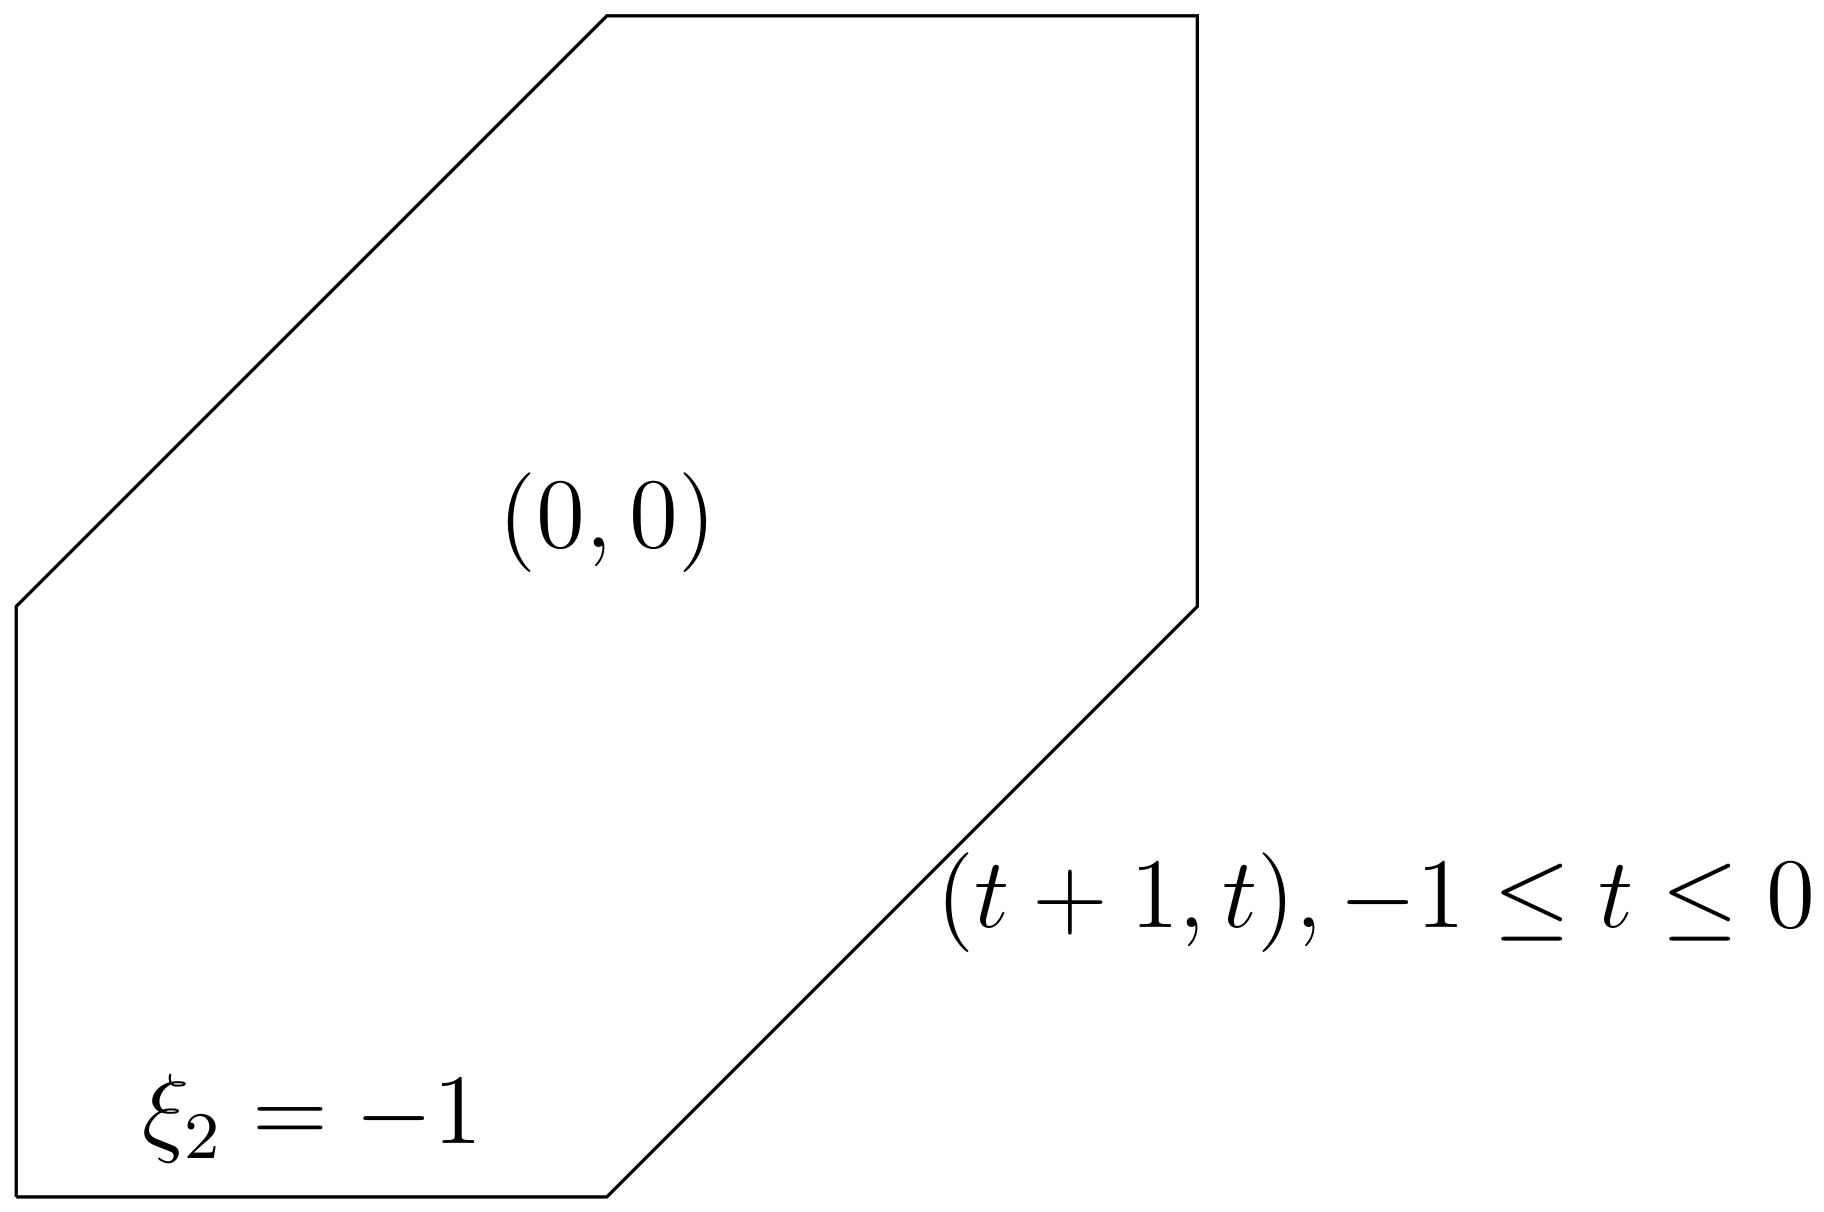
\includegraphics[width=0.52\textwidth]{figures/fig_1_2.png}
  \caption{由热带曲线界定的 $(0,0)$ 瓦片。（原书 p.26）}
  \label{fig:1-2}
\end{figure}

由周期性，这幅图铺满平面；由式~\eqref{eq:1-11}，$(m,n)$ 瓦片的斜率为
$m\xi_1+n\xi_2+\kappa(m\gamma'+n\gamma'')$。
\end{proof}

\transnote{证明只计算 $(0,0)$ 瓦片与相邻瓦片的交线；其余瓦片由 $\varphi$ 的周期性质（式~\eqref{eq:1-10}）平移得到。因此「蜂巢」是同一六边形沿 $\gamma'$、$\gamma''$ 两个方向铺成的。}

\medskip\noindent\textbf{概览：$(Y,v_0)$ 与 $\omega$ 的定义}\par

光滑流形 $Y$ 由环簇 $\tilde Y$ 的一部分取商得到；$\Gamma_B$ 通过全纯映射真不连续地作用。
其定义多面体为
\begin{equation}\label{eq:1-12}
\begin{gathered}
\Delta_{\tilde Y}:=\{(\xi_1,\xi_2,\eta)\in\R^3
  \mid\eta\ge\operatorname{Trop}(s)(\xi)\}\\
\Delta_Y:=(\Delta_{\tilde Y})|_{\eta\le T^l}/\Gamma_B\quad\text{其中}\\
\gamma\cdot(\xi_1,\xi_2,\eta):=(\xi_1+\gamma_1,\xi_2+\gamma_2,
  \eta-\kappa(\gamma)+\ip{\xi}{\lambda(\gamma)})\\
\because\operatorname{Trop}(s)(\xi+\gamma)=\operatorname{Trop}(s)(\xi)
  -\kappa(\gamma)+\ip{\xi}{\lambda(\gamma)}.
\end{gathered}
\end{equation}

多面体 $\Delta_{\tilde Y}$ 见图~\ref{fig:1-7}：$\eta$ 的下界由瓦片中央的表达式给出，
方向朝纸面外。复坐标将在下文讨论；此处先给出定义。

\transnote{作用 $\gamma\cdot$ 在 $(\xi_1,\xi_2)$ 方向平移，在 $\eta$ 方向平移并剪切，
恰好抵消 $\operatorname{Trop}(s)$ 在平移下的变化，所以图像在商下保持不变。这正是
$\Delta_Y$ 能良定义的原因。}

% ===== 原书 p.27 =====
\begin{definition}[{[AAK16][Definition 1.2]}]\label{def:syz-mirror}
称 $(Y,v_0)$ 为 $H=\Sigma_2$ 的广义 SYZ 镜像（generalized SYZ mirror）。
\end{definition}

\begin{remark}\label{rem:reverse-syz}
注意可以反向使用 SYZ：从 $Y$ 挖去一个除子后剩下的拉格朗日环面丛出发，把 $X$ 恢复为其
复镜像；参看 [AAK16, §8] 或 [CLL12]。
\end{remark}

\medskip\noindent\textbf{pair of pants：局部模型}\par

我们给出广义 SYZ 的一个示例，它是本文设定的局部模型。

\begin{example}[{[AAK16][§9.1]}]\label{ex:pants}
设 $H\subset V$ 是 $V=(\C^*)^2$ 中的 pair of pants（三孔球面）
$f(x_1,x_2):=1+x_1+x_2=0$。称之为 pair of pants，是因为
$x_1\in\C^*\setminus\{-1\}$，而柱面去掉一点正是 pair of pants。回忆
定义~\ref{def:tropicalization} 中 $\operatorname{Trop}(f)$ 的定义。
\end{example}

于是在 pair of pants 一例中 $\rho\equiv0$、$A=\{(0,0),(1,0),(0,1)\}$，因此
$\operatorname{Trop}(f)(\xi_1,\xi_2)=\max\{0,\xi_1,\xi_2\}$。若 $\xi_1,\xi_2<0$，
最大值为 $0$；若 $\xi_1>\xi_2>0$，最大值为 $\xi_1$；若 $\xi_2>\xi_1>0$，最大值为
$\xi_2$。所以 $\operatorname{Trop}(f)$ 的零点集（定义~\ref{def:vanishing}）如下图：

\begin{figure}[htbp]
  \centering
  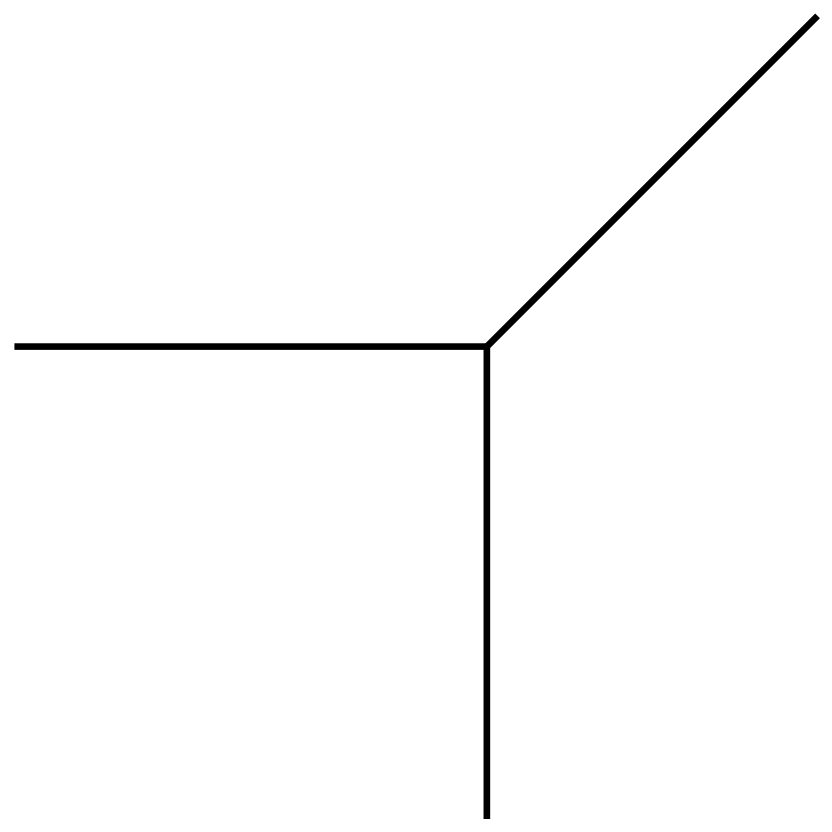
\includegraphics[width=0.2\textwidth]{figures/fig_1_3.png}
  \caption{$\operatorname{Trop}(1+x_1+x_2)=0$。（原书 p.27）}
  \label{fig:1-3}
\end{figure}

而矩多面体为 $\Delta:=\{(\xi,\eta)\mid\eta\ge\operatorname{Trop}(f)(\xi)\}
\subset\R^{n+1}$，如下图：

\begin{figure}[htbp]
  \centering
  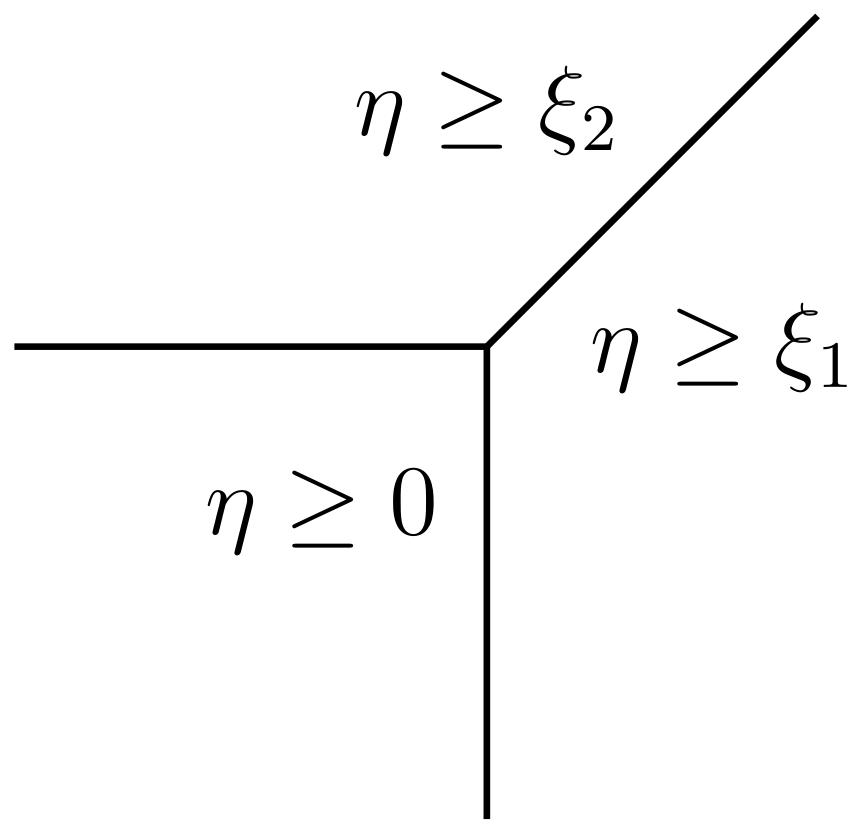
\includegraphics[width=0.26\textwidth]{figures/fig_1_4.png}
  \caption{矩多面体 $\subset\R^3$。（原书 p.27）}
  \label{fig:1-4}
\end{figure}

对 $(\xi_1,\xi_2,\eta)$ 作线性变换后，该多面体变为 $\R^3_{\ge0}$。相应的环簇是
$\operatorname{Spec}\C[x,y,z]=\C^3$。超势为 $v_0=xyz$，于是得到 pair of pants 的
预期镜像 $(\C^3,xyz)$。

\transnote{三点爆破的 $\C\PP^2$ 与 pair of pants 是同一局部模型的两种外观：前者是矩
多面体（六边形），后者是超曲面 $1+x_1+x_2=0$。多面体的每个顶点对应一个 $\C^3$
坐标卡，这正是后文用 $g_{xy}$ 在顶点附近插值的原因。}

% ===== 原书 p.28 =====
\medskip\noindent\textbf{$\omega$ 决定复坐标上的 $\Gamma_B$-作用}\par

我们要构造辛形式 $\omega$，使 1) 它是凯勒的，即与复环簇坐标继承的复结构相容；
2) $v_0:=xyz$ 是辛纤维丛；3) 它是环簇的，即在环面作用下不变。

由 3)，只需用复坐标的模长来定义辛形式。为保证 1)，局部地把 $\omega$ 写成某个凯勒势的
$\frac{i}{2\pi}\partial\bar\partial$，其中 $\partial\bar\partial$ 针对局部复环簇坐标。
为保证 2)，辛形式限制到每个纤维上都应是辛的。中心纤维是矩多面体由图~\ref{fig:1-5}
中六边形给出的环簇，再对 $\Gamma_B$ 取商。按 §1.3 的理论，它连同环簇
$\C\PP^2(3\text{ points})$（三点爆破）自带一个辛形式。离开 $v_0=0$ 但仍靠近多面体顶点
时，环簇局部地以例~\ref{ex:pants} 的局部模型 $(\C^3,xyz)$ 为模型。因此我们将用鼓包函数，
在 $\C\PP^2(3\text{ points})$ 的环簇辛形式与 $\C^3$ 上的标准形式之间插值。

\begin{figure}[htbp]
  \centering
  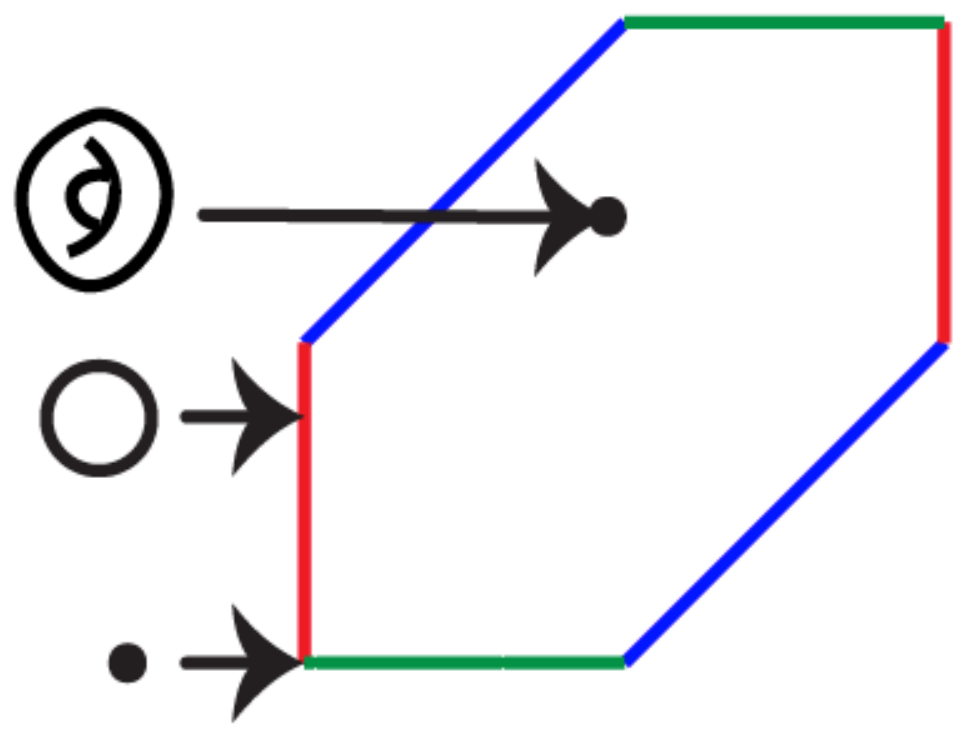
\includegraphics[width=0.28\textwidth]{figures/fig_1_5.png}
  \caption{$H=\Sigma_2$ 时 $(Y,v_0)$ 中心纤维的矩多面体。（原书 p.28）}
  \label{fig:1-5}
\end{figure}

下面解释降一维情形下辛形式构造的图示动机。

\begin{example}\label{ex:lower-dim}
设 $H$ 是椭圆曲线内的一点。此时多面体 $\Delta_{\tilde Y}$ 是二维的，可以画出来。
\end{example}

$v_0\colon\tilde Y\to\C$ 的纤维拓扑上是柱面；当 $|v_0|\to0$ 时，颈部周期性地被掐细，
退化为中心纤维上方的一串 $\PP^1$。在柱面最宽处，它看起来像球面的一部分，而 $\PP^1$
典范地带有富比尼–施图迪形式（Fubini--Study form）。另一方面，多面体顶点的邻域给出
坐标卡 $\C^2$，即 Lefschetz 纤维丛 $\C^2\to\C$、$(x,y)\mapsto xy$ 的局部图像，其中
柱面退化为以零点为顶点的锥。特别地，$\C^2$ 典范地带有标准形式 $\omega_{\mathrm{std}}$。
当环簇坐标很小时，由 $\log$ 的 Taylor 展开，富比尼–施图迪形式与标准形式近似相等。
因此在两个凯勒形式之间插值，即可构造辛形式。

% ===== 原书 p.29 =====
\begin{figure}[htbp]
  \centering
  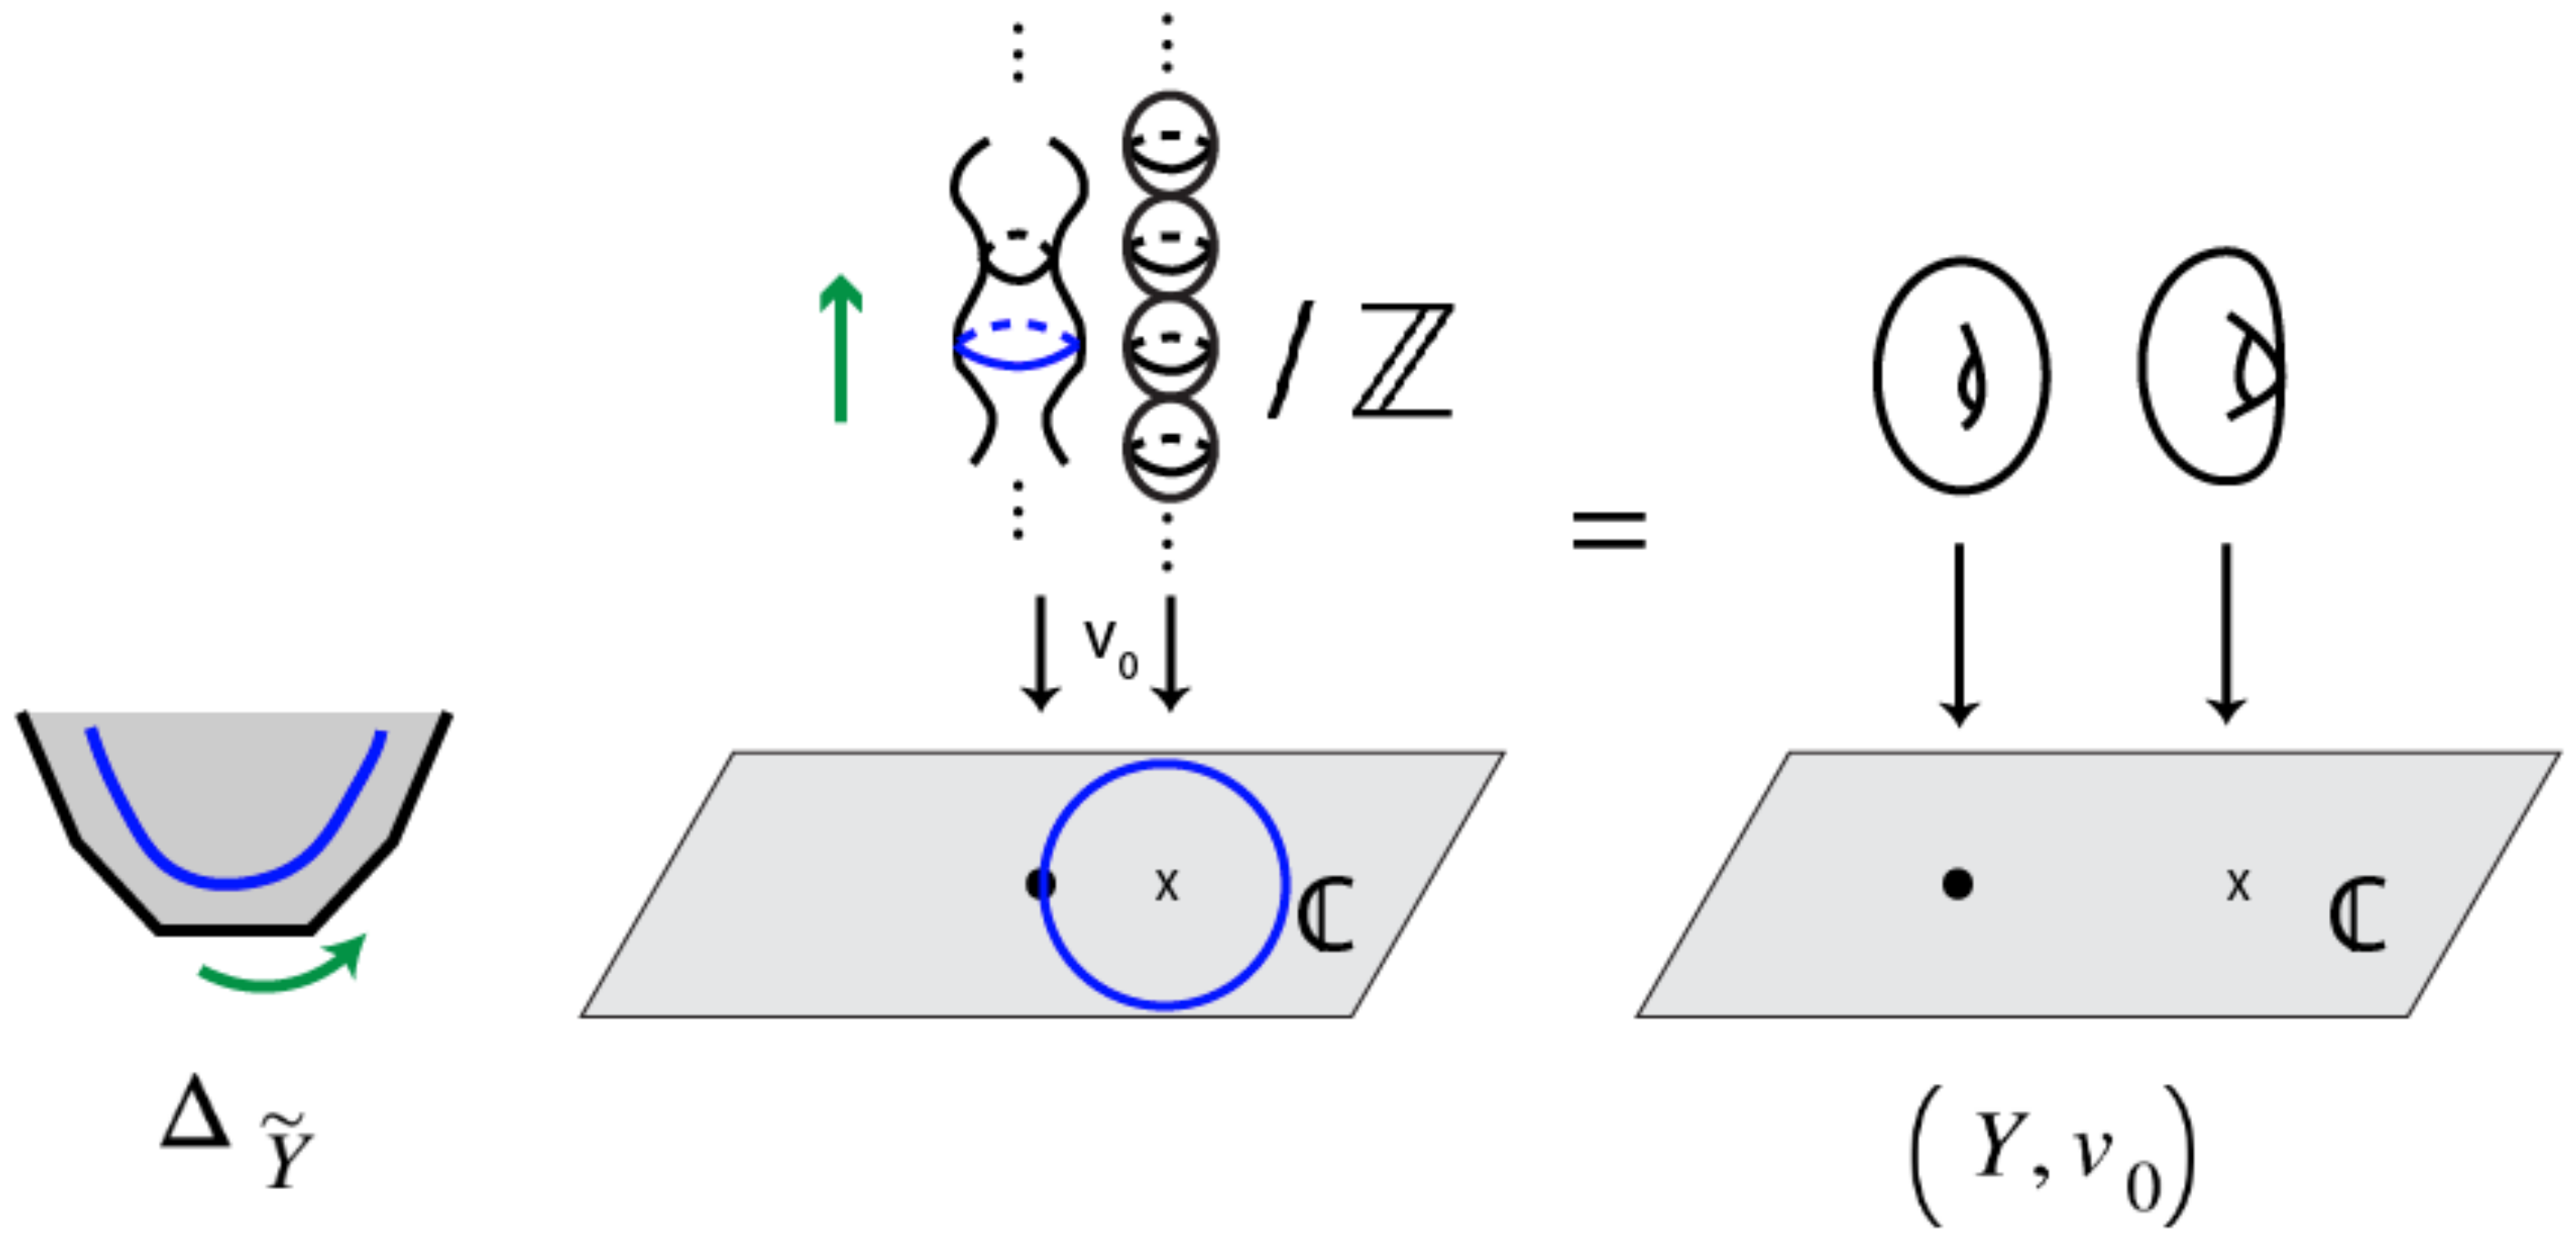
\includegraphics[width=0.8\textwidth]{figures/fig_1_6.png}
  \caption{降一维看，$\Delta_{\tilde Y}$ 的边界是一串 $\PP^1$ 的矩映射像。在多面体中
  $|v_0|$ 沿 $(0,1)$ 方向递增；在纤维丛 $v_0$ 中，$|v_0|$ 是底空间中圆的半径。
  （原书 p.29）}
  \label{fig:1-6}
\end{figure}

\begin{lemma}\label{lem:interpolation}
设 $r_x=|x|$，其余坐标同理，并设 $0<T\ll1$ 为常数。当 $H=\Sigma_2$ 时，
辛形式会在两种形式之间插值：一是顶点附近的局部坐标卡给出的 $(\C^3,\omega_{\mathrm{std}})$，
其凯勒势为 $\frac13T^2(r_x^2+r_y^2+r_z^2)$；
二是由六边形作为 $\C\PP^2$ 的三点爆破所诱导的环簇凯勒形式。
该凯勒势是「适当缩放的、对应格点的截面的平方和」的对数，如原书 1.3.29 的推论所述。
\end{lemma}

对某个 $(a,b,c)$，置
$g_{xy}:=\log(1+|T^ax|^2)(1+|T^by|^2)(1+|T^cxy|^2)$。
则 $(a,b,c)=(1,1,2)$ 具有正确的对称性，
使 $\omega$ 与 $\Gamma_B$-作用相容，并在商 $\tilde Y/\Gamma_B$ 上定义辛形式。

\transnote{引理中的「插值」有两层：一是在 $(\C^3,\omega_{\mathrm{std}})$ 与 $\C\PP^2$ 三点爆破的环簇形式之间插值；二是 $g_{xy}$ 中指数 $(a,b,c)$ 的选取要满足 $\Z/6$ 与 $\Gamma_B$ 的对称性。后文把这两层分别落实为鼓包函数与 $(a,b,c)=(1,1,2)$。}

\begin{remark}\label{rem:gxy-approx}
当 $Tr_x$ 与 $Tr_y$ 都很小时，有 $g_{xy}\approx(Tr_x)^2+(Tr_y)^2$。
\end{remark}

\begin{remark}\label{rem:figure17-scaling}
考察图~\ref{fig:1-7}，它画出本文的三维 $\Delta_{\tilde Y}$。
由环簇几何可知，$(x,y)$ 必定映到 $(y^{-1},xy)$ 的某个缩放，如图所示。
下文将定义合适的 $(\alpha,\beta)$，使该缩放为 $(x,y)\mapsto(T^\alpha y^{-1},T^\beta xy)$。
\end{remark}

\begin{definition}\label{def:G-action}
定义 $G=\Z/6\curvearrowright\tilde Y$，使六边形按如下方式顺时针旋转，
其中 $g$ 是 $G$ 的生成元：
\begin{equation}\label{eq:1-13}
g\cdot(x,y)=(T^\alpha y^{-1},T^\beta xy).
\end{equation}
更具体地说，$(x,y)$ 上的这一作用，通过指定它在 $v_0$ 的纤维上的限制，
决定了 $\tilde Y$ 上的作用；该纤维取一般纤维或退化的中心纤维。
换言之，$z$ 坐标上的作用是 $g\cdot z=T^{-\alpha-\beta}yz$，于是
$v_0=xyz\mapsto T^{\alpha+\beta-\alpha-\beta}y^{-1}\cdot xy\cdot yz=xyz$ 保持不变。
\end{definition}

\transnote{$\Z/6$-作用 $g$ 把六边形顺时针旋转一格；$\Gamma_B$ 则是由 $\gamma'$、$\gamma''$ 生成的平移群。两者在复坐标上的公式只差坐标置换 $\sigma_{g^n}$，务必分清「旋转」与「平移」两种操作。}

% ===== 原书 p.30 =====
\begin{figure}[htbp]
  \centering
  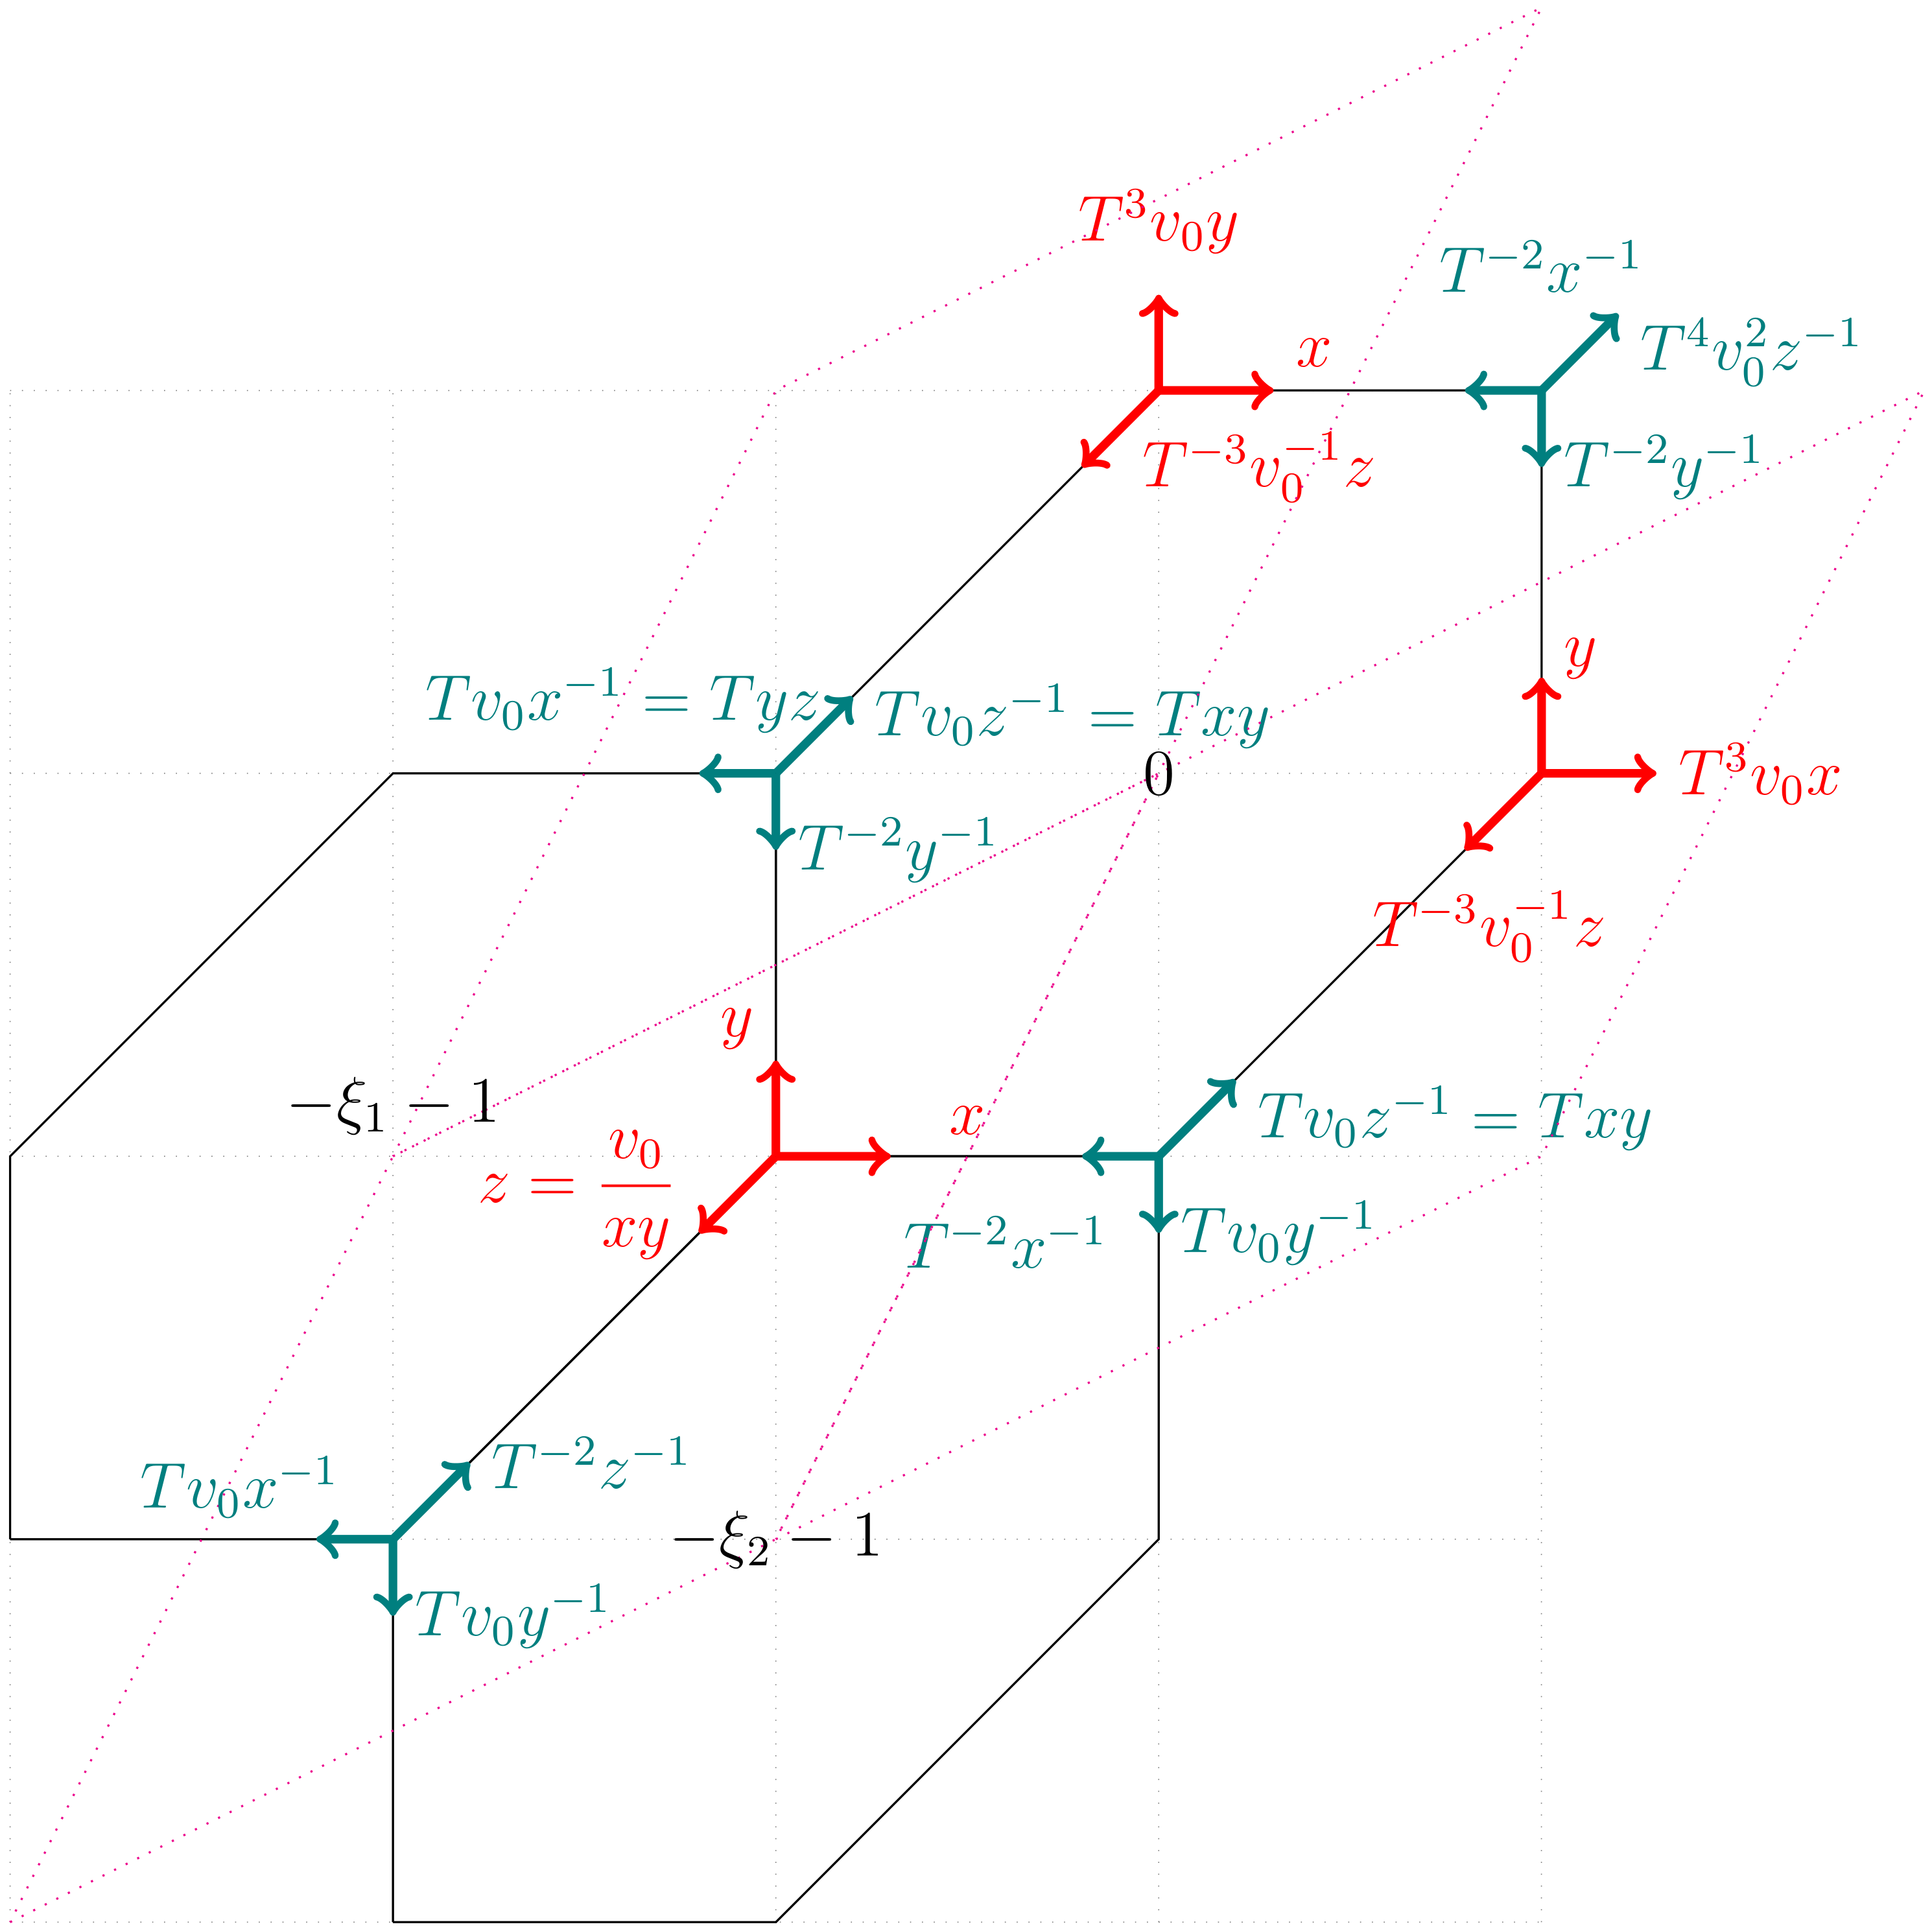
\includegraphics[width=0.8\textwidth]{figures/fig_1_7.png}
  \caption{$\Sigma_2$ 情形下 $\Delta_{\tilde Y}$ 的图示。图中坐标提示了
  $\Gamma_B$-作用，其动机与定义见后续各节。洋红色平行四边形是
  $\Gamma_B$-作用的基本域，中心为对角的 $\PP^1$。每个顶点是一个 $\C^3$ 坐标卡，
  坐标过渡将在引理~\ref{lem:interpolation} 中说明。瓦片中心处的表达式表示该瓦片上的
  $\eta\ge\varphi(\xi)=-\xi_1-1$ 一类不等式；六条边的方程表明瓦片 $(0,0)$ 由
  $(\xi_1,\xi_2)\in\{(\xi_1,\xi_2)\mid-1\le\xi_1,\xi_2,-\xi_1+\xi_2\le1\}$ 给出。
  （原书 p.30）}
  \label{fig:1-7}
\end{figure}

\begin{claim}\label{clm:area-one}
在 $G$ 作用下，若 $g_{xy}$ 映到的凯勒势只相差一个调和函数，
即相差 $\log|T^{\alpha/2}y|^2$，则沿 $y$ 轴的 $\PP^1$ 的辛面积为 $1$。
\end{claim}

\begin{proof}
我们沿 $z$ 轴计算。由对称性，沿 $y$ 轴的计算与之类似，故只需考虑前者。
注意由 Stokes 定理，沿 $z$ 轴的 $\PP^1$ 辛面积为 $1$。
回忆 $\PP^1$ 有开覆盖 $U_0,U_\infty$，坐标卡 $\varphi_0$ 与 $\varphi_1$
分别把 $[z_0:z_1]$ 送到 $z_1/z_0$ 与 $z_0/z_1$。
我们要把 $\PP^1$ 上的积分拆到这两个卡上，但只取到两卡相交之处，否则积分区域过大。
于是 $z$ 是 $\varphi_0(U_0)\cong\C$ 上的坐标，
% [Tutor Note: 原文此处称坐标卡为 φ1，而下式与后文均写作 φ∞；疑为同一张卡的笔误，保留原样。]

% ===== 原书 p.31 =====
它在 $\varphi_\infty(U_\infty)$ 上是 $1/(T^\alpha z)$，并且
$|z|=|1/T^\alpha z|\Longrightarrow|z|=1/T^{\alpha/2}$。
令 $D_0$ 为 $\varphi_0(U_0)$ 中的圆盘，$D_\infty$ 为另一卡中对应的圆盘。
设 $F_0,F_\infty$ 为两卡中的凯勒势。
\begin{align*}
\int_{\PP^1}\frac{i}{2\pi}\partial\bar\partial F
&=\frac{i}{2\pi}\Bigl[\int_{\varphi_0^{-1}(D_0)}d(\bar\partial F)
 +\int_{-\varphi_\infty^{-1}(D_\infty)}d(\bar\partial F)\Bigr]\\
&=\frac{i}{2\pi}\Bigl[\int_{\partial D_0}\bar\partial(\varphi_0^{-1})^*F
 -\int_{\partial D_\infty}\bar\partial(\varphi_\infty^{-1})^*F\Bigr]\\
&=\frac{i}{2\pi}\int_{C_{1/T^{\alpha/2}}}\bar\partial(F_0-F_\infty)\\
&=\frac{i}{2\pi}\int_{C_{1/T^{\alpha/2}}}\bar\partial\log(|T^{\alpha/2}z|^2)
 =\frac{i}{2\pi}\int_{C_{1/T^{\alpha/2}}}\frac{T^\alpha z\,d\bar z}{|T^{\alpha/2}z|^2}\\
&=\frac{i}{2\pi}\int_0^{2\pi}e^{i\theta}(-i)e^{-i\theta}\,d\theta=1.
\end{align*}
\end{proof}

\transnote{只需沿 $z$ 轴计算，其余两轴由 $(x,y,z)$ 的轮换对称性得到。积分拆到 $U_0$ 与 $U_\infty$ 两张卡，交线是圆 $C_{1/T^{\alpha/2}}$；最后一步为 $\int_0^{2\pi}e^{i\theta}(-i)e^{-i\theta}\,d\theta=2\pi$，再乘 $i/2\pi$ 得 $1$。}

\begin{proof}[{主引理~\ref{lem:interpolation} 的证明}]
\begin{gather*}
g^*\log(1+|T^ax|^2)(1+|T^by|^2)(1+|T^cxy|^2)\\
=\log(1+|T^{a+\alpha}y^{-1}|^2)(1+|T^{b+\beta}xy|^2)(1+|T^{c+\alpha+\beta}x|^2),\\
g_{xy}=\log(1+|T^ax|^2)(1+|T^by|^2)(1+|T^cxy|^2).
\end{gather*}
我们预期两个势相差 $\log|T^by|^2$，因为 $y$ 在 $g$ 下变为 $y^{-1}$。
比较指数得
\begin{gather*}
b=-a-\alpha,\\
a=c+\alpha+\beta,\\
c=b+\beta.
\end{gather*}
这里有 5 个未知量与 3 个方程，故应能化为 2 个未知量。
具体地，把 $(a,b,c)$ 用 $(\alpha,\beta)$ 表示，再要求 $x\leftrightarrow y$ 对称，
即令 $a=b$，从而用 $\beta$ 确定 $\alpha$。
\begin{align*}
a&=c+\alpha+\beta=(b+\beta)+\alpha+\beta=(-a-\alpha)+\alpha+2\beta\\
\Longrightarrow a&=\beta\\
\Longrightarrow b&=-\alpha-\beta\\
a=b\ \therefore\ \alpha&=-2\beta\\
\Longrightarrow c&=b+\beta=2\beta\\
\therefore\ g_{xy}&=\log(1+|T^\beta x|^2)(1+|T^\beta y|^2)(1+|T^{2\beta}xy|^2).
\end{align*}
取 $\beta=1$ $\Longrightarrow$ $g_{xy}=\log(1+|Tx|^2)(1+|Ty|^2)(1+|T^2xy|^2)$。

% ===== 原书 p.32 =====
由于取 $\beta=1$，可见沿 $x$ 轴（由对称性，沿 $y$、$z$ 轴亦然）复坐标的模改变 $T^{-2}$。
于是施加 $g$ 时 $y$ 的值变大；但那里新的坐标系（后文记作 $(x'',y'',z'')$）
与原 $(x,y,z)$ 处一样取小值。
\end{proof}

\transnote{「$y$ 的值变大」说的是旧坐标在新卡中的量级，相差 $T^{-2}$；
换到新卡 $(x'',y'',z'')$ 后各坐标仍取小值。读图~\ref{fig:1-7} 时不宜把两者混为一谈。}

下一节将说明为何 $(\alpha,\beta)=(-2,1)$ 与 $g\cdot(x,y)=(T^{-2}y^{-1},Txy)$
给出图~\ref{fig:1-7} 所画的 $\Gamma_B$-作用。
由此便可定义 $Y$ 为商 $\tilde Y/\Gamma_B$；
其中 $\tilde Y$ 由 $\Delta_{\tilde Y}$ 按 §1.3 所述构造。

\medskip\noindent\textbf{$Y$ 的定义}\par

\begin{remark}[约定]\label{rem:convention}
约定：在图~\ref{fig:1-7} 中向上、向右移动为负方向。
因为 $T\ll1$ 的正幂次使坐标值变小，而坐标值变小对应沿群作用的负方向移动。
也就是说，$\gamma'$ 与 $\gamma''$ 的作用分别把坐标 $(x,y,z)$ 送到
图~\ref{fig:1-7} 中以 $(-2,-1)$ 与 $(-1,-2)$ 为中心的卡。
\end{remark}

\transnote{图~\ref{fig:1-7} 中坐标的指向与 $T$ 的幂次相反：$T\ll1$ 时 $T$ 的正幂次让坐标值变小，所以图上「向上、向右」对应群作用的负方向。核对 $\gamma'$、$\gamma''$ 的像之前，先确认这一约定。}

\begin{definition}[$\Gamma_B$-作用的定义]\label{def:GammaB-action}
$(x,y,z)$ 上的 $\Gamma_B$-作用可由定义~\ref{def:G-action} 中定义的 $\Z/6$-作用读出。
即 $g^2$ 像 $-\gamma''$ 那样，把 $(x,y,z)$ 送到以 $(\xi_1,\xi_2)=(1,2)$ 为中心的坐标系；
但它是通过旋转来置换坐标方向的。
事实上，$g$ 把 $(x,y,z)\mapsto(T^{-2}y^{-1},Txy,Tyz)$。
为抵消 $g$ 中的这一置换、使方向保持不变，即
$(x,y,z)\mapsto(Tyz,T^{-2}y^{-1},Txy)=(Tv_0x^{-1},T^{-2}y^{-1},Tv_0z^{-1})$；
对施加 $g^2$ 所得的坐标作同样的置换，即可定义 $\Gamma_B$-作用：
\[
(-\gamma'')\cdot(x,y,z):=(x,T^3v_0y,T^{-3}v_0^{-1}z).
\]
\end{definition}

\begin{definition}[{$Y$ 的定义}]\label{def:Y}
现在可以用商 $\tilde Y/\Gamma_B$ 定义 $Y$：
\begin{equation}\label{eq:1-14}
\begin{gathered}
\Delta_{\tilde Y}:=\{(\xi_1,\xi_2,\eta)\in\R^3\mid\eta\ge\operatorname{Trop}(s)(\xi)\}\\
\Delta_Y:=(\Delta_{\tilde Y})|_{\eta\le T^l}/\Gamma_B\quad\text{其中式~\eqref{eq:1-10} 表明}\\
\gamma\cdot(\xi_1,\xi_2,\eta):=(\xi_1+\gamma_1,\xi_2+\gamma_2,\eta-\kappa(\gamma)+\ip{\xi}{\lambda(\gamma)}).
\end{gathered}
\end{equation}
\end{definition}

$\Delta_{\tilde Y}$ 的每个顶点对应三个复坐标，可以用 $(x,y,z)$（以及 $v_0=xyz$）写出。
图~\ref{fig:1-7} 列出了这些坐标；为清楚起见，我们在此把它们收集为坐标卡 $U_{n,g^k}$。
其中 $\gamma=n_1\gamma'+n_2\gamma''$ 表示所看瓦片在 $\Delta_{\tilde Y}$ 中投影到前两个坐标后的中心，
$g^k$ 表示绕六边形走到了何处。
$g^k$ 只用来索引坐标卡；但如定义~\ref{def:GammaB-action} 所述，
坐标是 $g^k\cdot(x,y,z)$ 的置换，所以下标主要用于索引。过渡映射为
\[
(x,y,z)\mapsto\sigma_{g^n}\cdot(g^n\circ\gamma)\cdot(x,y,z),
\qquad n\in\Z/6,\ \gamma\in\Gamma_B.
\]

% ===== 原书 p.33 =====
其中 $\sigma_{g^n}$ 是坐标的某个置换，依赖于 $n$，见定义~\ref{def:GammaB-action}。
从 $(x,y,z)$ 出发，沿 $(0,0)$ 瓦片顺时针走：
\begin{itemize}[leftmargin=2.2em,itemsep=0.25em]
\item $U_{0,g^0}$：$(x,y,z)$。
\item $U_{0,g}$：$(Tv_0x^{-1},T^{-2}y^{-1},Tv_0z^{-1})=:(x'',y'',z'')$。
\item $U_{0,g^2}$：$(x,T^3v_0y,T^{-3}v_0^{-1}z)=:(-\gamma'')\cdot(x,y,z)$。
\item $U_{0,g^3}$：$(T^{-2}x^{-1},T^{-2}y^{-1},T^4v_0^2z^{-1})$。
\item $U_{0,g^4}$：$(T^3v_0x,y,T^{-3}v_0^{-1}z)=:(-\gamma')\cdot(x,y,z)$。
\item $U_{0,g^5}$：$(T^{-2}x^{-1},Tv_0y^{-1},Tv_0z^{-1})=:(x',y',z')$。
\item 沿 $z$ 轴走，可到 $(-1,0)$ 瓦片中的 $g^{-1}$ 顶点：
\item $U_{(-1,0),g^{-1}}$：$(Tv_0x^{-1},Tv_0y^{-1},T^{-2}z^{-1})=:(x''',y''',z''')$。
\end{itemize}

于是：当 $|v_0|=T^l$、$T\ll1$ 且 $l$ 充分小时，$\Gamma_B$ 真不连续地全纯作用，
故商是良定义的复流形 $Y$。
% [Tutor Note: 原文作「l sufficiently small」；但要使 |v0|=T^l 很小（T<<1），应需 l 充分大。保留原样，登记为疑点。]

\begin{proof}[{由 $\Z/6$-作用计算坐标}]
由于 $g\cdot(x,y)=(T^{-2}y^{-1},Txy)$，把群作用施加两次得
\[
(x,y)\sim(T^{-2}y^{-1},Txy)\sim
\bigl(T^{-2}(T^{-1}x^{-1}y^{-1}),T(T^{-2}T^{-1})(Txy)\bigr)
=(T^{-3}x^{-1}y^{-1},x).
\]
% [Tutor Note: 原件第二分量写作 T(T^{-2}T^{-1})(Txy)，代入得 T^{-1}xy，与右侧的 x 不符；疑应为 T(T^{-2}y^{-1})(Txy)=x。保留原样，登记为疑点。]
特别地，$\Gamma_B$ 固定 $v_0=xyz$，故可把变换后的 $y$ 坐标改写为 $T^3v_0y$，
从而在适当的置换 $\sigma_{g^2}$ 之后得到 $\gamma''$-作用：
\[
\sigma_{g^2}\cdot g^2\cdot(x,y,z)=:-\gamma''\cdot(x,y,z)
=(x,T^3v_0y,T^{-3}v_0^{-1}z).
\]
$\gamma'$ 的计算与之类似。为求坐标系 $(x''',y''',z''')$，
先沿 $\gamma'$ 的作用向左下方移动，进入 $(0,-1)$ 瓦片，
再用 $g^{-1}$ 旋转，最后施加适当的置换。
由于 $g^{-1}\cdot(x,y)=(Txy,T^{-2}x^{-1})$，得
$g^{-1}\cdot(x,y,z)=(Tv_0z^{-1},T^{-2}x^{-1},Tv_0y^{-1})$。于是
\begin{align*}
\gamma'\cdot(x,y,z)&=(T^{-3}v_0^{-1}x,y,T^3v_0z),\\
g^{-1}\cdot(T^{-3}v_0^{-1}x,y,T^3v_0z)
&=\bigl(Tv_0(T^3v_0z)^{-1},T^{-2}(T^{-3}v_0^{-1}x)^{-1},Tv_0y^{-1}\bigr)\\
&=(T^{-2}z^{-1},Tv_0x^{-1},Tv_0y^{-1}),\\
\therefore\ (x''',y''',z''')
&:=\sigma_{g^{-1}}\cdot g^{-1}\cdot\gamma'\cdot(x,y,z)\\
&=(Tv_0x^{-1},Tv_0y^{-1},T^{-2}z^{-1}).
\end{align*}
\end{proof}

上面所列各卡中其余坐标的计算与此类似。

% ===== 原书 p.34 =====
\begin{remark}\label{rem:symmetry-told-structure}
注意，$\omega$ 所需的对称性质告诉我们需要何种复结构（它给出乘积复结构）；
由镜像对称，这将对应 $X$ 的 A 模型上某个特定的辛形式。
我们在定义~\ref{def:Y} 的列表中，用新的带撇变量标记图~\ref{fig:1-7} 的部分绿色坐标卡坐标。
\end{remark}

\begin{corollary}[{$Y$ 上的复结构}]\label{cor:complex-structure}
复结构这样得到：先把多面体 $\Delta_{\tilde Y}$ 每个顶点的环簇卡，
通过把 $(x,y,z)$ 与各其他顶点的新坐标系粘合而等同起来。
然后按 $\Gamma_B$-作用取商；该作用缩放坐标而保持 $v_0=xyz$，
故商上 $v_0$ 的纤维是阿贝尔簇。用复坐标写出，$\Gamma_B$-作用为
\[
(x,y,z)\sim(T^3v_0x,y,T^{-3}v_0^{-1}z),\qquad
(x,y,z)\sim(x,T^3v_0y,T^{-3}v_0^{-1}z).
\]
\end{corollary}

\begin{remark}\label{rem:gluing-rescaling}
注意，在按 $\Gamma_B$-作用取商之前，把所有环簇卡粘好后纤维会是 $(\C^*)^2$。
复坐标中的 $\Gamma_B$-作用，对应从 $\Delta_{\tilde Y}$ 过渡到
$\Delta_Y=\Delta_{\tilde Y}/\Gamma_B$。
我们仍按多面体等同单项式来粘环簇卡，但允许在粘合复坐标时发生缩放。
（例如低一维：对 $\C^*\ni x\mapsto Tx$，把单位圆与半径 $T$ 的圆粘起来，得到环面。）
\end{remark}

\begin{remark}[术语]\label{rem:terminology}
环簇 $\tilde Y$ 被 [KL19] 称为「无穷型」（infinite-type）环簇，
因为它的面有无穷多个；那里环簇除子的邻域，
等同于我们限制到 $|v_0|$ 小（即 $\eta$ 小）的情形。
\end{remark}

\begin{definition}[超势]\label{def:superpotential}
超势 $v_0$ 是全纯函数 $Y\to\C$，定义为
\begin{equation}\label{eq:1-15}
v_0(x,y,z):=xyz,
\end{equation}
它在 $Y$ 上是良定义的全局函数，因为它在 $\Gamma_B$-作用下不变。
\end{definition}

\begin{remark}\label{rem:symplectic-fibration}
我们将在第 2 章为 $v_0$ 配上辛纤维丛结构，
再在 §4.1 为它配上深谷–Seidel 范畴。
\end{remark}

\begin{remark}\label{rem:AAK16-comparison}
这里的复坐标上的 $\Gamma_B$-作用与 [AAK16, §10.2] 所述不同。
这意味着 $Y$ 作为 $X$ 的镜像，所用的辛形式与其论文中的不同。那里的复结构是
\begin{equation}\label{eq:1-16}
\boldsymbol{v}^m\sim v_0^{\ip{\lambda(\gamma)}{m}}T^{\ip{\gamma}{m}}\boldsymbol{v}^m,
\end{equation}
其中用复坐标 $\boldsymbol{v}=(v_1,v_2)$。于是置 $(x,y,z)=(v_1^{-1},v_2^{-1},v_0v_1v_2)$，
其复结构来自如下 $\Gamma_B$-作用：
\begin{gather*}
\gamma'\cdot(x,y,z)=(T^{-2}v_0^{-1}x,T^{-1}y,T^3v_0z),\\
\gamma''\cdot(x,y,z)=(T^{-1}x,T^{-2}v_0^{-1}y,T^3v_0z).
\end{gather*}
\end{remark}

% ===== 原书 p.35 =====
\medskip\noindent\textbf{把多面体划分为区域}\par

回忆图~\ref{fig:1-7} 的多面体 $\Delta_{\tilde Y}$。
我们先在一个顶点的邻域内定义 $\omega$。
它用 $\tilde Y$ 上一组新的局部实径向与角向坐标 $d$ 与 $\theta$ 定义，
在图~\ref{fig:1-9} 的每个划分区域内各有一套。

这些划分由下列变量给出。固定 $|v_0|(=|xyz|)=T^l$，
其中 $T\ll1$，$l$ 是大的正常数。
在图~\ref{fig:1-9} 的支集内，$r_x,r_y,r_z\ll1$，
故式~\eqref{eq:1-18} 的近似成立。

定义函数 $\phi_x,\phi_y,\phi_z$，它们对理解后续计算至关重要。
\begin{equation}\label{eq:1-17}
\begin{gathered}
\phi_x(x,y,z):=\log_T\frac{1+|Tx|^2}{1+|T^2yz|^2},\\
\phi_y(x,y,z):=\log_T\frac{1+|Ty|^2}{1+|T^2xz|^2},\\
\phi_z(x,y,z):=\log_T\frac{1+|Tz|^2}{1+|T^2xy|^2}.
\end{gathered}
\end{equation}

现在可以定义计算中要用的局部径向与角向坐标。
它们的下标表示其定义所在的是图 1.4 的哪个区域。
% [Tutor Note: 此处划分区域画在图 1.8/1.9，原文「图 1.4」疑为「图 1.9」之误。保留原样，登记为疑点。]

\begin{figure}[htbp]
  \centering
  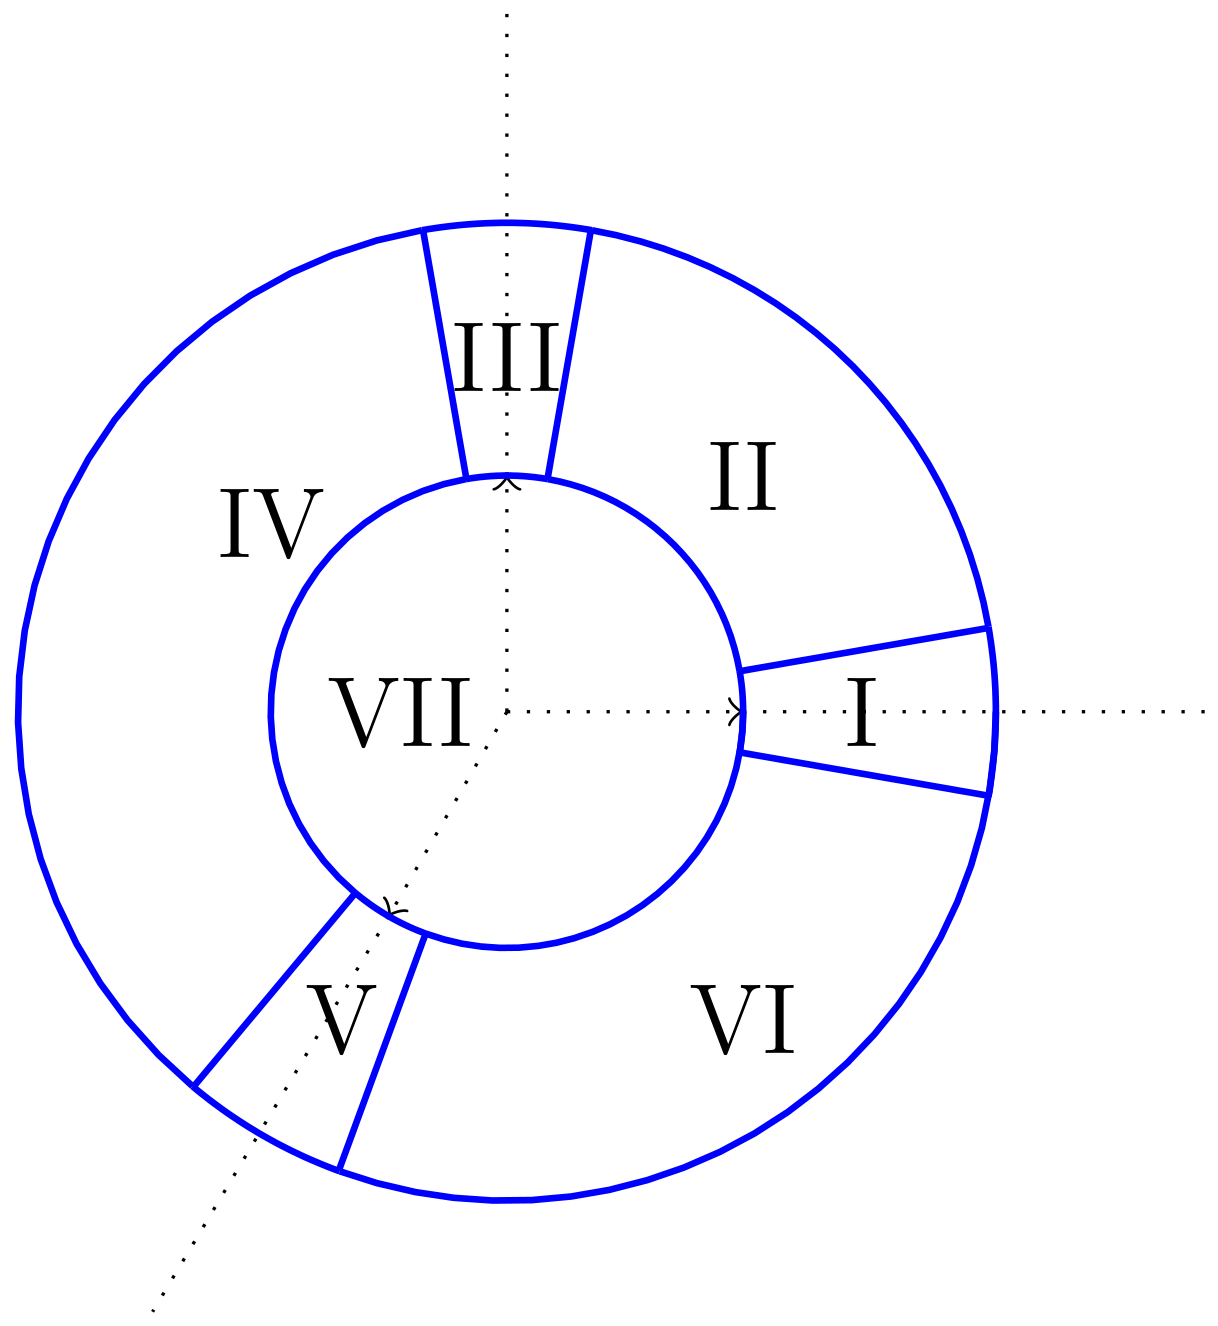
\includegraphics[width=0.3\textwidth]{figures/fig_1_8.png}
  \caption{围绕一个顶点划分 $\Delta_{\tilde Y}$ 中的区域。（原书 p.35）}
  \label{fig:1-8}
\end{figure}

% ===== 原书 p.36 =====
\begin{equation}\label{eq:1-18}
\begin{gathered}
d_I:=\phi_x-\frac12(\phi_y+\phi_z)\\
=\log_T\Biggl(\frac{1+|Tx|^2}{1+|T^2v_0x^{-1}|^2}\Bigg/
\sqrt{\frac{1+|Ty|^2}{1+|T^2v_0y^{-1}|^2}\cdot
\frac{1+|Tz|^2}{1+|T^2v_0z^{-1}|^2}}\Biggr)\\
\approx(Tr_x)^2-\frac12\bigl((Tr_y)^2+(Tr_z)^2\bigr)
\qquad\text{当 }r_x,r_y,r_z\ll1\text{ 时}\\
\theta_I:=\phi_y-\phi_z\\
=\log_T\Bigl(\frac{1+|Ty|^2}{1+|Tz|^2}\cdot\frac{1+|T^2xy|^2}{1+|T^2xz|^2}\Bigr)
\approx(Tr_y)^2-(Tr_z)^2.
\end{gathered}
\end{equation}

\par\noindent\rule{\textwidth}{0.4pt}\par

\begin{equation}\label{eq:1-19}
\begin{gathered}
d_{IIA}:=\phi_x-\frac12(\phi_y+\phi_z)+\frac32\alpha_6(\theta_{II})\cdot\phi_y
\approx T^2\Bigl[r_x^2-\frac12(r_y^2+r_z^2)+\frac32\alpha_6(\theta_{II})\cdot r_y^2\Bigr]\\
d_{IIB}:=\phi_x+\phi_y-\frac12\phi_z,\\
d_{IIC}:=\phi_y-\frac12(\phi_x+\phi_z)+\frac32\alpha_6(-\theta_{II})\cdot\phi_x,\\
\theta_{II}:=\log_T r_y-\log_T r_x.
\end{gathered}
\end{equation}

其中 $\alpha_6$ 是角向上的截断函数，将在下文定义。最后定义
\begin{equation}\label{eq:1-20}
\begin{gathered}
d_{III}:=\phi_y-\frac12(\phi_x+\phi_z),\qquad
\theta_{III}:=\phi_z-\phi_x,\\
d_V:=\phi_z-\frac12(\phi_x+\phi_y),\qquad
\theta_V:=\phi_x-\phi_y.
\end{gathered}
\end{equation}

沿图~\ref{fig:1-9} 上图各轴，$(1,0)$ 方向有 $r_y=r_z<r_x$，
$(0,1)$ 方向有 $r_x=r_z<r_y$，$(-1,-1)$ 方向有 $r_x=r_y<r_z$。

\begin{definition}[{图 1.9 中各区域的定义}]\label{def:regions}
划分区域 I 的曲线为：左右两条上 $d_I$ 为常数，上下两条上 $\theta_I$ 为常数。
可分别近似为 $r_x$ 为常数与 $r_y$ 为常数，
同时另两个变量变化而 $|xyz|=T^l$ 保持不变。
在区域 VII 的原点处 $|x|=|y|=|z|=T^{l/3}$，
因为三个坐标相等且乘积为 $|v_0|=T^l$。
取 $p$ 充分大，我们定义如下。
\end{definition}

% ===== 原书 p.37 =====
\begin{figure}[htbp]
  \centering
  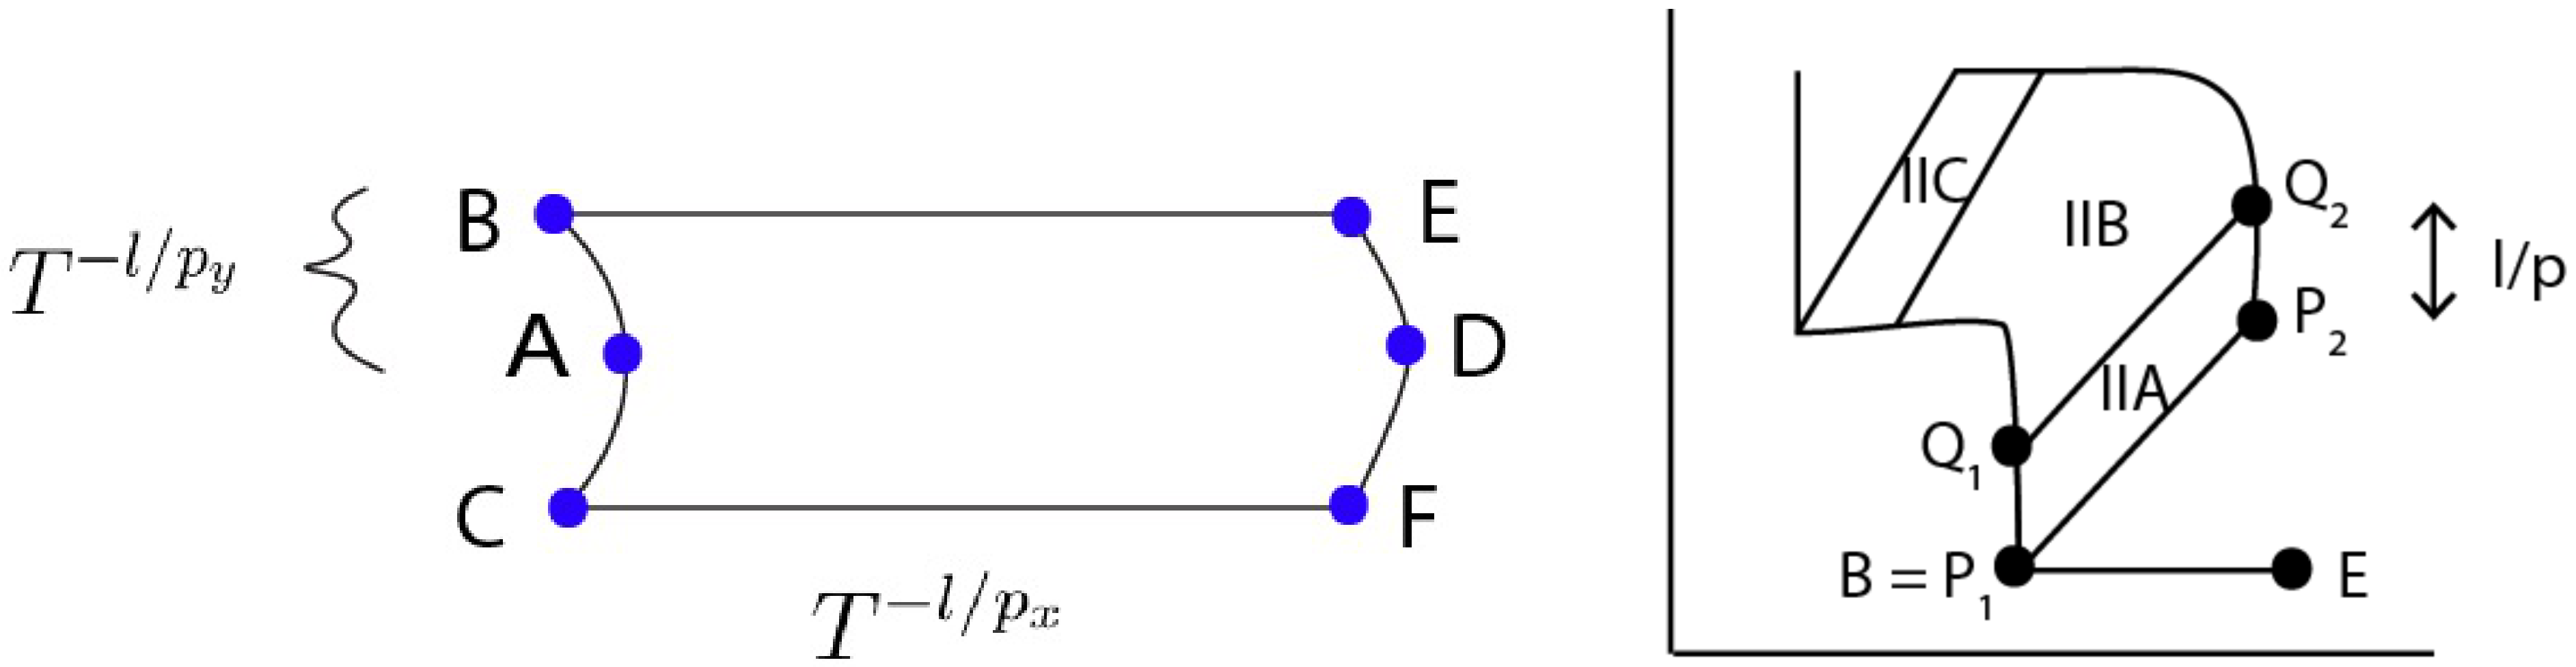
\includegraphics[width=0.95\textwidth]{figures/fig_1_9.png}
  \caption{左、右两图分别是区域 I 与区域 II 的放大。（原书 p.37）}
  \label{fig:1-9}
\end{figure}

\noindent\textbf{区域 I}
\begin{itemize}[leftmargin=2.2em,itemsep=0.25em]
\item $A(r_x,r_y,r_z)=(T^{l/4},T^{3l/8},T^{3l/8})$。
\item $B(r_x,r_y,r_z)\approx(T^{l/4},T^{3l/8-l/p},T^{3l/8+l/p})$。
\item $C(r_x,r_y,r_z)\approx(T^{l/4},T^{3l/8+l/p},T^{3l/8-l/p})$。
\item $D(r_x,r_y,r_z)=(T^{l/4-l/p},T^{3l/8+l/2p},T^{3l/8+l/2p})$。
此处 $r_x$ 已增大，而 $r_y=r_z$ 保持不变。
\item $E(r_x,r_y,r_z)\approx(T^{l/4-l/p},T^{3l/8-l/p},T^{3l/8+2l/p})$。
\item $F(r_x,r_y,r_z)\approx(T^{l/4-l/p},T^{3l/8+2l/p},T^{3l/8-l/p})$。
\end{itemize}

划分区域 II 的曲线为：沿径向向外的直线 $\theta_{II}$ 为常数，
沿角向曲线 $d_{IIA}$ 或 $d_{IIB}$ 为常数。
注意此处 $d_{IIA}$ 为常数近似于 $r_x$ 为常数。

\noindent\textbf{区域 II}
\begin{itemize}[leftmargin=2.2em,itemsep=0.25em]
\item $P_1=B\approx(T^{l/4},T^{3l/8-l/p},T^{3l/8+l/p})$。
\item $P_2\approx(T^{l/4-l/p},T^{3l/8-2l/p},T^{3l/8+3l/p})$。
\end{itemize}
这是因为从 $P_1$ 到 $P_2$ 的窄条上 $\theta_{II}=\log_T r_y-\log_T r_x$ 为常数；
而 $P_2$ 由沿 $d_I\approx(Tr_x)^2$ 常数的方向把 $E$ 上移得到，
故 $r_x(P_2)\approx T^{l/4-l/p}$。于是 $\theta_{II}$ 为常数给出
\begin{align*}
\theta_{II}(P_1)&\approx3l/8-l/p-l/4=l/8-l/p\\
&=\theta_{II}(P_2)\approx\log_T r_y-(l/4-l/p)\\
\Longrightarrow\ \log_T r_y&\approx3l/8-2l/p.
\end{align*}

% ===== 原书 p.38 =====
\begin{itemize}[leftmargin=2.2em,itemsep=0.25em]
\item $Q_1\approx(T^{l/4},T^{3l/8-2l/p},T^{3l/8+2l/p})$。
从 $P_1$ 沿 $d_{IIA}$ 常数到 $Q_1$，$r_y$ 乘以 $T^{-l/p}$，而 $r_x$ 近似不变。
\item $Q_2\approx(T^{l/4-l/p},T^{3l/8-3l/p},T^{3l/8+4l/p})$。
从 $Q_1$ 到 $Q_2$，$\theta_{II}$ 为常数；在 $Q_1$ 处
$\theta_{II}(Q_1)\approx3l/8-2l/p-l/4=l/8-2l/p$。
从 $P_2$ 到 $Q_2$，$r_x$ 近似不变，故 $Q_2$ 处 $\log_T r_x$ 近似为 $l/4-l/p$，于是
\[
\log_T r_y\approx(l/8-2l/p)+(l/4-l/p)=3l/8-3l/p.
\]
\end{itemize}
$r_z$ 坐标由 $r_xr_yr_z=T^l$ 确定。

现在终于得到关于 $p$ 的条件。我们希望区域 IIA 中处处 $r_x\gg r_y$，
使 $d_{IIA}$ 的等值线大致如所画，且 $d_{IIA}$ 的近似成立。
看 $Q_1$，这意味着 $T^{l/4}\gg T^{3l/8-2l/p}$；$Q_2$ 给出同样的限制。
故需 $1/8-2/p>0$，即 $p>16$。例如取 $p=17$。

其余区域由对称性定义。

\transnote{$p$ 的作用是把区域 IIA 的坐标细化到可分辨的程度；条件 $p>16$ 来自 $r_x\gg r_y$ 的要求，即比较 $Q_1$ 处的 $T^{l/4}$ 与 $T^{3l/8-2l/p}$。取 $p=17$ 只是方便的选取，不影响几何。}

\subsection{辛形式的定义}

现在定义 $H=\Sigma_2$ 情形下的辛形式。

\begin{figure}[htbp]
  \centering
  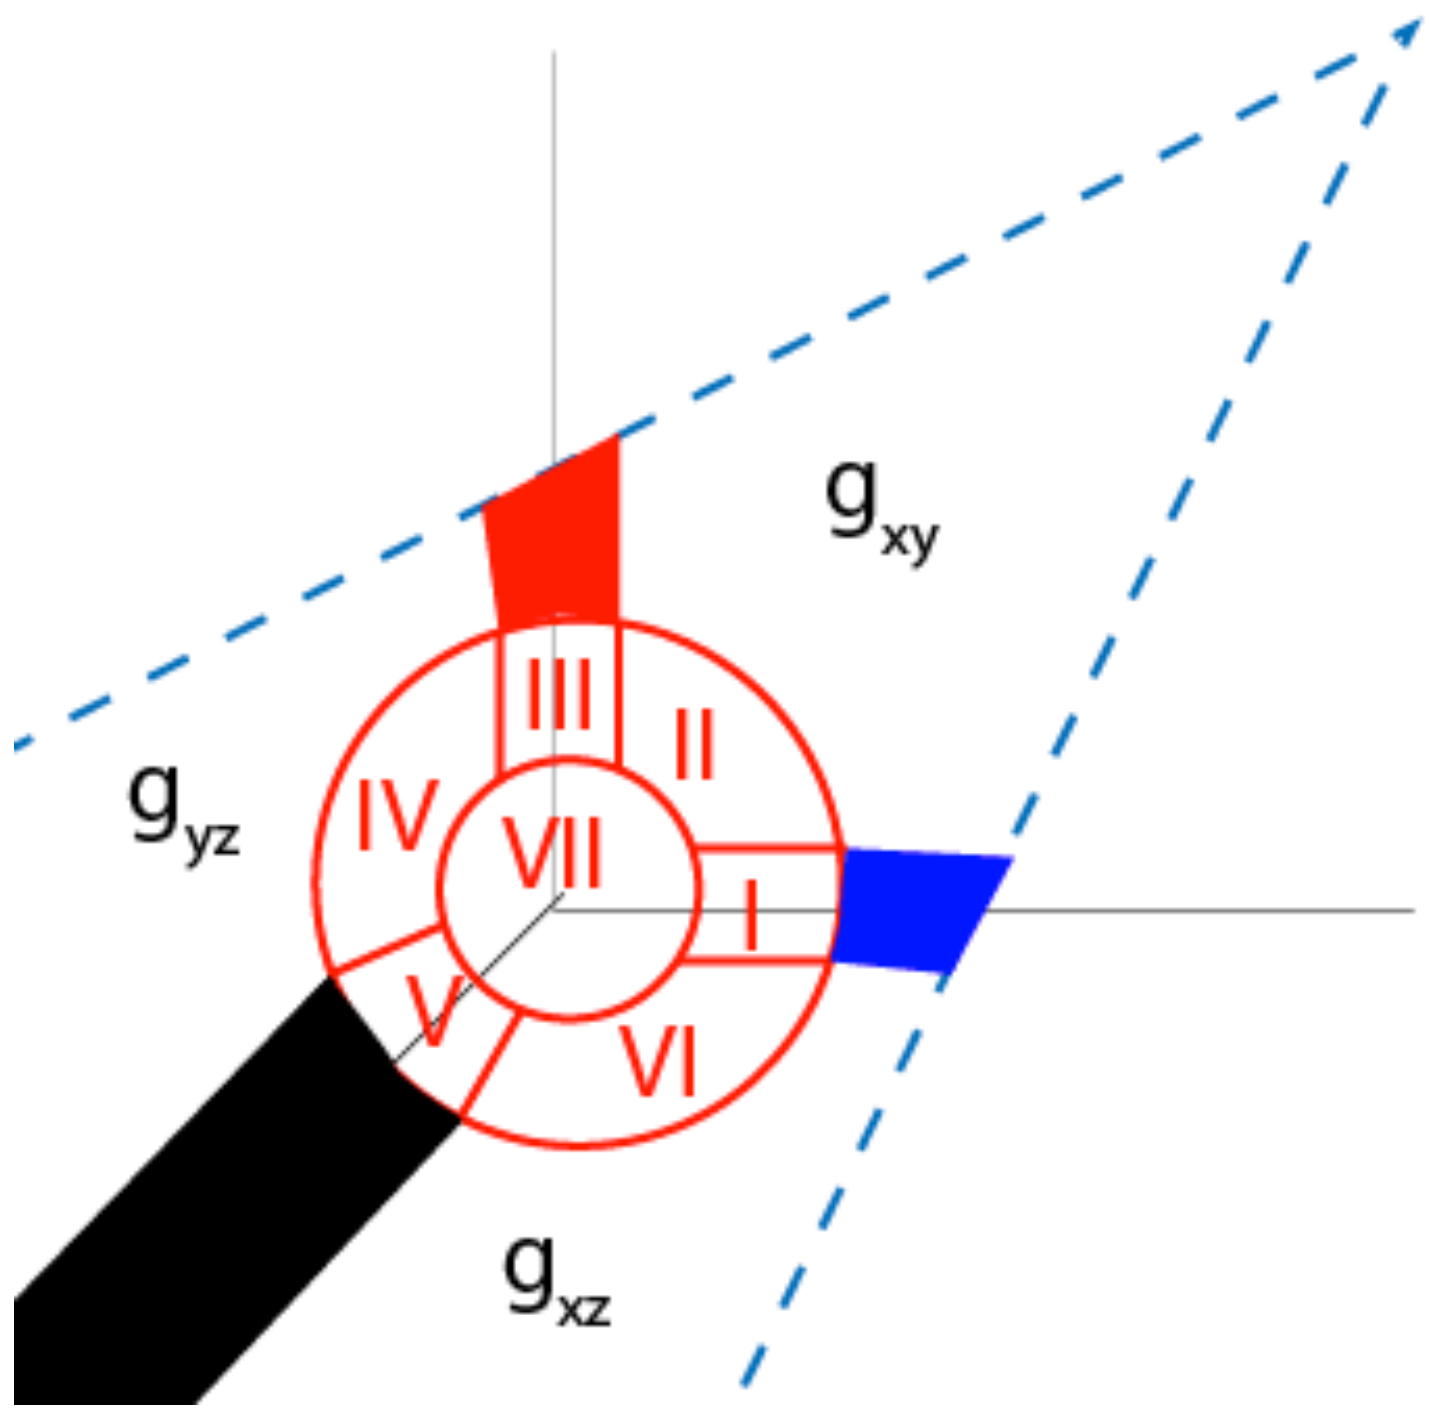
\includegraphics[width=0.38\textwidth]{figures/fig_1_10.png}
  \caption{在三个势之间插值：$F=\alpha_1g_{xy}+\alpha_2g_{xz}+(1-\alpha_1-\alpha_2)g_{yz}$，
  $0\le\alpha_1,\alpha_2\le1$。区域 VII 是 $\alpha_1=\alpha_2=1/3$ 之处；
  由对数近似，$F=\frac13(g_{xy}+g_{xz}+g_{yz})\approx\frac23((Tr_x)^2+(Tr_y)^2+(Tr_z)^2)$。
  （原书 p.38）}
  \label{fig:1-10}
\end{figure}

% ===== 原书 p.39 =====
\begin{definition}[辛形式的定义]\label{def:symplectic-form}
置 $\omega=\frac{i}{2\pi}F$，其中 $F$ 局部地由式~\eqref{eq:1-18} 的坐标定义如下：
\begin{equation}\label{eq:1-21}
\begin{gathered}
g_{yz}=\log(1+|Ty|^2)(1+|Tz|^2)(1+|T^2yz|^2),\\
g_{xz}=\log(1+|Tx|^2)(1+|Tz|^2)(1+|T^2xz|^2),\\
g_{xy}=\log(1+|Tx|^2)(1+|Ty|^2)(1+|T^2xy|^2).
\end{gathered}
\end{equation}
引入新的鼓包函数 $\alpha_3,\dots,\alpha_6$ 如下：
\[
\frac23\le\alpha_3(d_I)=\alpha_1+\alpha_2\le1,\qquad
-\frac12\le\alpha_4(\theta_I)\le\frac12,\qquad
0\le\alpha_5(d_I)\le1,\qquad
0\le\alpha_6(\theta_{II})\le1,
\]
\[
\alpha_4(\theta_I)\cdot\alpha_5(d_I)=\frac12(\alpha_1-\alpha_2).
\]
这些鼓包函数光滑、作为指定变量的函数递增，
且在定义域两端附近取所给界值的常数。
我们还要求 $\alpha_4$ 是奇函数。
关于这些鼓包函数性质的解释，见下小节「定义的动机」。
现在定义如下；注意 $g_{xz}-g_{yz}=\phi_x-\phi_y$，且 $(x,y,z)$ 的轮换同理：
\begin{equation}\label{eq:1-22}
\begin{gathered}
\text{图 1.10 中的区域 } g_{\bullet}\text{：分别对应 }F=g_{xy},\ F=g_{yz},\ F=g_{xz}\\
\text{区域 I：}\quad F=g_{yz}+\alpha_3(d_I)d_I+\alpha_4(\theta_I)\alpha_5(d_I)\theta_I\\
\text{区域 IIA：}\quad F=g_{yz}-\alpha_6(\theta_{II})\phi_y+\alpha_3(d_{IIA})d_{IIA}\\
+\frac12\alpha_5(d_{IIA})\bigl(\phi_y-\phi_z-\alpha_6(\theta_{II})\phi_y\bigr)\\
\text{区域 IIB：}\quad F=(g_{yz}-\phi_y)+\alpha_3(d_{IIB})d_{IIB}-\frac12\alpha_5(d_{IIB})\phi_z\\
\text{区域 IIC：}\quad F=g_{xz}-\alpha_6(-\theta_{II})\phi_x+\alpha_3(d_{IIC})d_{IIC}\\
+\frac12\alpha_5(d_{IIC})\bigl(\phi_x-\phi_z-\alpha_6(-\theta_{II})\phi_x\bigr)\\
\text{区域 I 到区域 IIA：}\quad F=g_{yz}+\alpha_3(d_I)\cdot d_I+\frac12\alpha_5(d_I)\cdot\theta_I\\
=g_{yz}+\alpha_3(d_{IIA})d_{IIA}+\frac12\alpha_5(d_{IIA})\cdot\theta_I\\
\text{区域 VII：}\quad F=\frac13(g_{xy}+g_{xz}+g_{yz})
\end{gathered}
\end{equation}

这些公式在边界处互相匹配，因此可以用 $(x,y,z)$ 的置换，
把区域 III–VI 像 I、II 那样由对称性定义。
例如可以验证：区域 IIA 的公式在 $\alpha_3=\frac23$、$\alpha_5=0$ 时与区域 VII 的公式一致；
在 $\alpha_6=0$、$\alpha_4=\frac12$ 时与区域 I 的一致；
在 $\alpha_6=1$ 时与区域 IIB 的一致；在 $\alpha_3=\alpha_5=1$ 时与 $g_{xy}$ 一致。
其余区域的计算类似。
\end{definition}

沿坐标轴（即染成红、蓝、黑色的区域），
我们用与区域 I、III、V 相同的公式、取 $\alpha_3\equiv1$，在相应的 $g_{\bullet}$ 之间插值。
例如沿 $r_x$ 轴（蓝色区域），公式为
$F=\frac12(g_{xy}+g_{xz})+\alpha_4(\theta_I)(g_{xy}-g_{xz})$；其余边类似。

\transnote{$\alpha_4\cdot\alpha_5=\frac12(\alpha_1-\alpha_2)$ 把两个鼓包函数捆绑在一起：$\alpha_5$ 控制径向支撑，$\alpha_4$ 控制角向变化。边界匹配正是靠这一乘积条件与 $\alpha_4$ 的奇性。}

% ===== 原书 p.40 =====
由于凯勒势是局部定义的，且在 $(\xi_1,\xi_2)$ 坐标中原点邻域内关于 $(x,y,z)$ 对称，
我们可以要求凯勒形式在先前所述 $\Z/6$-作用与 $\Gamma_B$-作用下都不变，从而处处定义它。
这一相容性条件在下面的断言~\ref{clm:descends} 中验证。

辛形式的定义到此完成。

\medskip\noindent\textbf{定义的动机}\par

我们可以重新整理 $F$ 的初始表达式中依赖于 $\alpha_1,\alpha_2$ 的项，
以说明 $\alpha_3$ 与 $\alpha_4\cdot\alpha_5$ 的定义，以及各区域中 $d$ 与 $\theta$ 的定义。
$\alpha_6$ 的选取与区域 II 中的变量，是为了在两侧（即区域 I 与 III）$F$ 的定义之间插值。
\begin{align*}
F&=\alpha_1g_{xy}+\alpha_2g_{xz}+(1-\alpha_1-\alpha_2)g_{yz}\\
&=\alpha_1\log(1+|Tx|^2)(1+|Ty|^2)(1+|T^2xy|^2)
+\alpha_2\log(1+|Tz|^2)(1+|Tx|^2)(1+|T^2xz|^2)\\
&\quad+(1-\alpha_1-\alpha_2)\log(1+|Tz|^2)(1+|Ty|^2)(1+|T^2yz|^2)\\
&=g_{yz}+(\alpha_1+\alpha_2)\phi_x
-\Bigl(\frac{\alpha_1+\alpha_2}{2}-\frac{\alpha_1-\alpha_2}{2}\Bigr)\cdot\phi_y
-\Bigl(\frac{\alpha_1+\alpha_2}{2}+\frac{\alpha_1-\alpha_2}{2}\Bigr)\cdot\phi_z\\
&=g_{yz}+(\alpha_1+\alpha_2)\bigl(\phi_x-\tfrac12(\phi_y+\phi_z)\bigr)
+\tfrac12(\alpha_1-\alpha_2)(\phi_y-\phi_z).
\end{align*}

注意 $\alpha_1,\alpha_2,1-\alpha_1-\alpha_2$ 并不对称，但三者应被对称地对待，
故如上合并。换言之，把 $(\alpha_1,\alpha_2)$ 看作向量并旋转 $\pi/4$，得到与
\[
\begin{pmatrix}1&-1\\1&1\end{pmatrix}
\begin{pmatrix}\alpha_1\\\alpha_2\end{pmatrix}
=\begin{pmatrix}\alpha_1-\alpha_2\\\alpha_1+\alpha_2\end{pmatrix}
\]
成比例的向量。

\transnote{把 $\alpha_1g_{xy}+\alpha_2g_{xz}+(1-\alpha_1-\alpha_2)g_{yz}$ 按三个 $\log$ 因子重新分组；$g_{yz}$ 之外的项恰好组合成 $\phi_x-\frac12(\phi_y+\phi_z)$ 与 $\phi_y-\phi_z$，这就是 $d_I$ 与 $\theta_I$ 的来源。}

定义 $\alpha_3=\alpha_1+\alpha_2$。为得到其界，我们考虑几何以及 $\alpha_1,\alpha_2$ 的变化。
在中心区域 VII 中 $\alpha_1=\alpha_2=1/3$。
沿 $r_x$ 方向穿过区域 I 到达尽头时，不应有 $g_{yz}$ 贡献，
即那里 $\alpha_3=\alpha_1+\alpha_2=1$。于是区域 I 中 $\alpha_3$ 从 $2/3$ 变到 $1$。

我们用 $\alpha_1-\alpha_2$ 定义角向变化的鼓包函数 $\alpha_4$，
其角向变量记作 $\theta_I$，定义见下文。这里有一处需要注意。
在区域 I 起点 $\alpha_1=\alpha_2=1/3$，故沿角 $\theta_I$ 走时 $\alpha_1-\alpha_2$ 始终为 $0$；
但在区域 I 末端，从底部的 $(\alpha_1,\alpha_2)=(0,1)$ 走到顶部的 $(1,0)$，
于是 $\alpha_1-\alpha_2$ 在 $-1$ 与 $1$ 之间变化。
因此需把 $\alpha_4(\theta_I)$ 乘以另一个鼓包函数 $\alpha_5(d_I)$；
后者从 $0$ 变到 $1$，依赖于随 $r_x$ 增大而增大的变量 $d_I$，下文将定义。
于是我们缩放了 $\alpha_4$ 的变化区间。出于对称性，要求 $\alpha_4$ 是奇函数。
% ===== 原书 p.41 =====
令 $\alpha_4\cdot\alpha_5=\frac12(\alpha_1-\alpha_2)$，于是
\[
F=g_{yz}+\alpha_3\bigl(\phi_x-\tfrac12(\phi_y+\phi_z)\bigr)+\alpha_4\cdot\alpha_5(\phi_y-\phi_z).
\]

后续计算的关键在于：鼓包函数会乘以它所依赖的变量。
$\alpha_i$ 依据「绕圆走了多远」（角向）与「离中心多远」（径向）变化。
于是我们引入一组坐标 $d$ 与 $\theta$，它们可从上面 $F$ 的表达式读出：
$d_I=\phi_x-\frac12(\phi_y+\phi_z)$，$\theta_I=\phi_y-\phi_z$。
下面从几何上说明它们为何合理。

我们想构造一个辛形式，使其矩多面体由 Delzant 定理与环簇多面体相同。
从图中能读出的是 $r_x,r_y,r_z$ 彼此如何比较；
即使无法确定其值，也可观察它们的相对大小。
特别地，在图~\ref{fig:1-11} 中可见：$T^2(r_y^2-r_z^2)$ 沿向上的竖直方向增大，
$(Tr_x)^2$ 沿向右的水平方向增大。
这启发了我们对角向与径向变量的选取；这些变量可用首阶项近似。

\begin{figure}[htbp]
  \centering
  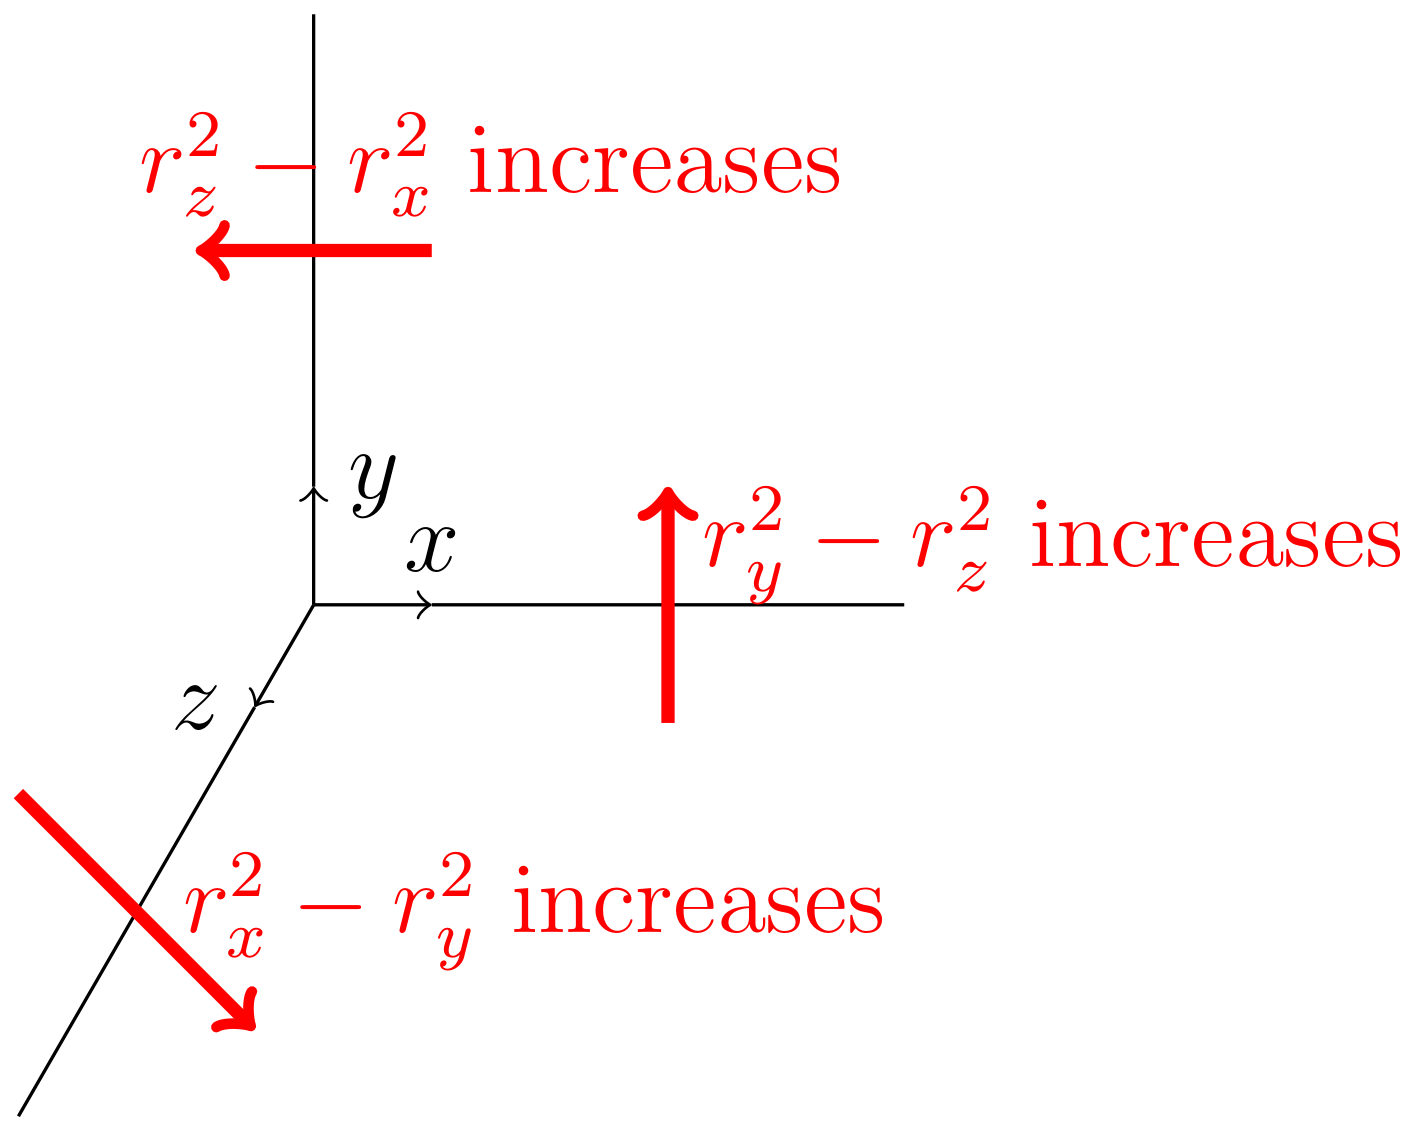
\includegraphics[width=0.4\textwidth]{figures/fig_1_11.png}
  \caption{三条角向如何变化。（原书 p.41）}
  \label{fig:1-11}
\end{figure}

在区域 I 中，$d$ 应随 $x$ 增大。
具体地，$d_I:=\phi_x-\frac12(\phi_y+\phi_z)$ 仍随 $x$ 增大，
因为区域 I 开始时 $r_x\gg r_y,r_z$。
（由于 $v_0=xyz$，固定纤维时 $|x|$ 增大意味着 $|yz|$ 相应减小。）

对角度方向，注意在表达式 $\phi_x:=\log(1+|Tx|^2)/(1+|T^2yz|^2)$ 中，
首阶项是 $|Tx|^2$。于是如上所述，$\theta_I=\phi_y-\phi_z$ 应是角向坐标，从而得到
\[
F=g_{yz}+\alpha_3(d_I)\cdot d_I+\alpha_4(\theta_I)\cdot\alpha_5(d_I)\cdot\theta_I.
\]
至此定义了区域 I 中的凯勒势。由 $(x,y,z)$ 的对称性，它也定义了区域 III 与 V 中对应的势。
随后区域 II 在这些势之间插值。

% ===== 原书 p.42 =====
\medskip\noindent\textbf{$\omega$ 延拓过中心纤维并下降到 $Y$}\par

由于 $\omega$ 的构造，该形式延拓为全空间上的形式，包含零纤维。
若在顶点周围画一个圆盘并考虑其上所有 $|v_0|$ 值，
就得到 $\C^3$ 中的一块，其凯勒形式在 $r_x,r_y,r_z$ 小时近似标准辛形式；
也就是说，我们移植了 $(\C^3,xyz)$ 模型纤维丛的一部分，
而它是光滑流形、有良定义的辛形式。
若在六边形中心取一个圆盘形区域，那里只有一个凯勒势起作用，
再考虑其上所有 $|v_0|$，就得到纤维中的模型环簇凯勒形式；
再加上来自纤维丛 $v_0$ 底空间的一项，便得到乘积辛形式。

在这两者之间插值的区域中，得到两个正定凯勒势的凸线性组合。
特别地，可取 $\epsilon$ 充分小，使给这两个度量之一加上 $\epsilon$ 不影响正定性。
然后固定 $l$ 的取值，使某些 $|v_0|=T^l$ 时下文所述所有鼓包函数导数都小于 $\epsilon$。
之后可令 $|v_0|=T^{l'}$ 趋于零，而界仍然成立：若对 $l$ 成立，则 $l'\to\infty$ 时只会更小。
换言之，一旦为鼓包函数导数留出足够空间，
就可以定义它们在所有 $v_0\to0$ 的纤维上有相同的支集，并在其余部分为常数。

此外，$\omega$ 以 $\Gamma_B$-不变（也以 $\Z/6$-不变）的方式延拓到整个 $\tilde Y$：
用群作用在定义~\ref{def:Y} 引入的其他坐标卡 $U_{n,g^k}$ 中定义它。
于是这些公式在卡的重叠处相符，给出 $\tilde Y$ 上良定义的 2-形式。
进一步，它如下下降到商 $Y$ 上良定义的 2-形式。

\begin{claim}\label{clm:descends}
形式 $\omega$ 下降到商 $Y=\tilde Y/\Gamma_B$ 上良定义的 2-形式。
\end{claim}

\begin{proof}
上面已见 $\omega$ 的局部模型良定义，因为所有局部定义在边界处一致；
这一点在定义~\ref{def:symplectic-form} 末尾已指出。
此外，在 $\Delta_{\tilde Y}$ 的每个顶点与六边形瓦片中心粘合坐标卡 $U_{n,g^k}$
（见定义~\ref{def:Y}）时，公式一致。
例如引理~\ref{lem:interpolation} 证明 $g_{xy}$ 在 $\Z/6$-作用下对称。
最后，沿边的定义必须相容。换言之，取 $\alpha_3=\alpha_5=1$，
从区域 I、III、V 延拓到图 ?? 中染成黑、红、蓝的阴影区域时，变换是相容的。
% [Tutor Note: 原文作「of Figure ??」，是坏引用；按上下文应为图 1.10。保留原样，登记为疑点。]
由对称性，只需沿 $r_z$ 轴检验。
按定义~\ref{def:Y} 的记号，这是主卡 $U_{0,g^0}$（坐标 $(x,y,z)$）
与坐标卡 $U_{(-1,0),g^{-1}}$（坐标 $(x''',y''',z''')=(Tyz,Txz,T^{-2}z^{-1})$）之间的变换。

设 $F$ 为未加撇坐标中辛形式的凯勒势，$F'''$ 为三撇坐标中的凯勒势。
在我们考虑的区域，$F$ 由区域 V 的公式在 $\alpha_3=\alpha_5=1$ 时给出。

% ===== 原书 p.43 =====
\begin{align*}
F_V&=g_{xy}+d_V+\alpha_4(\theta_V)\cdot\theta_V\\
g_{xy}+d_V&=\log_T(1+|Tx|^2)(1+|Ty|^2)(1+|T^2xy|^2)\cdot\\
&\quad\Biggl(\frac{1+|Tz|^2}{1+|T^2xy|^2}\Bigg/
\sqrt{\frac{1+|T^2xz|^2}{1+|Ty|^2}\cdot\frac{1+|T^2yz|^2}{1+|Tx|^2}}\Biggr)\\
&=\frac12\log_T(1+|Tx|^2)(1+|Ty|^2)(1+|T^2xz|^2)(1+|T^2yz|^2)
+\log_T(1+|Tz|^2)\\
\theta_V&=\phi_x-\phi_y\\
\therefore\ g'''_{xy}&=\Bigl(\frac12\log_T(1+|T^2yz|^2)(1+|T^2xz|^2)(1+|Ty|^2)(1+|Tx|^2)
+\log_T(1+|T^{-1}z^{-1}|^2)\Bigr)\\
&\quad+\alpha_4(-\theta_V)\cdot(-\theta_V)\\
&=g_{xy}-\log_T(|Tz|^2).
\end{align*}
最后等号成立：第一项中，用 $(x,y,z)$ 与 $(x''',y''',z''')$ 之间的坐标变换作拉回，
只是置换因子；第二项用 $\alpha_4(-\theta)=-\alpha_4(\theta)$。
又注意在该坐标卡下 $\theta_V'''$ 对应 $-\theta_V$。
于是从一个卡到另一个卡需加 $\log_T(|Tz|^2)$；
它是调和函数，因为 $\log(Tz)$ 全纯而其共轭反全纯。
\end{proof}

\transnote{「延拓过中心纤维」与「下降到商」是两件不同的事：前者用 $(\C^3,xyz)$ 局部模型补上零纤维处的定义，后者验证 $\Gamma_B$-不变性。至于 $\omega$ 闭且非退化、以及正定性，引理~\ref{lem:symplectic-on-Y} 把它们留到第 2 章。}

\begin{lemma}\label{lem:symplectic-on-Y}
$\omega$ 的定义给出 $Y$ 上良定义的辛形式。
\end{lemma}

其完整证明在下一章，将证明正定性。
